\documentclass[a4paper]{article}

\usepackage{fullpage} % Package to use full page
\usepackage{parskip} % Package to tweak paragraph skipping
\usepackage{tikz} % Package for drawing
\usepackage{amsmath}
\usepackage{hyperref}
\usepackage[utf8]{inputenc}
\usepackage{graphicx}
\usepackage{lmodern}
\usepackage[MeX]{polski}
\usepackage[T1]{fontenc}

\title{Notatki z kursu Inżynieria Oprogramowania}
\author{Małgorzata Dymek}
\date{2018/19, semestr letni}

\begin{document}
\maketitle


\section{Definicje i podstawowe zadania}
\textbf{Inżynieria oprogramowania}
    \begin{itemize}
        \item dziedzina wiedzy zajmująca się wszystkimi zagadnieniami związanymi z produkcją oprogramowania
        \begin{itemize}
            \item analiza
            \item wymagania
            \item projektowanie
            \item wdrożenie
            \item ewolucja systemu
        \end{itemize}

        \item zastosowanie  systematycznego, zdyscyplinowanego, ilościowego podejścia do rozwoju, eksploatacji i utrzymania
        oprogramowania, czyli zastosowanie inżynierskiego podejścia do oprogramowania
    \end{itemize}

\textbf{Podstawowe pojęcia}
    \begin{itemize}
        \item Uczestnicy i role.
        \item Systemy i modele.
        \item Produkt - wewnętrzny lub docelowy.
        \begin{itemize}
            \item specyfikacja
            \item podręcnzik użytkowania
            \item scenariusze przypadków użycia
            \item raport o statusie projektu
            \item podręcznik testera
        \end{itemize}
        \item Aktywności, zadania i zasoby - na przykład:
        \begin{itemize}
            \item zbieranie wymagań
            \item analiza
            \item realizacja przypadku użycia
            \item zaprojektowanie schematu bazy danych, systemu, obiektów
            \item implementacja
            \item testowanie
        \end{itemize}
        \item Notacje, metody i metodologie.
        \item Wymagania - funkcjonalne i niefunkcjonalne.
    \end{itemize}


Zarządzanie tworzeniem oprogramowania poprzez \textbf{aktywności}, celem dostarczenie wysokiej jakości
produktu na czas i zgodnie z zaplanowanym budżetem. Aktywności - koncentrują się na planowaniu
projektu, monitorowaniu jego statusu, śledzeniu zmian i koordynowaniu wykorzystania zasobów. Obejmują m.in.:
    \begin{itemize}
        \item komunikację
        \item zarządzanie konfiugracją
        \item zarządzanie projektem
        \item cykl życiowy oprogramowania
    \end{itemize}


\section {Wprowadzenie do UMLa, przypadki użycia}

\textbf{UML - Unified Modelling Language}
    \begin{itemize}
        \item rodzina notacji graficznych
        \item służy do opisywania i projektowania stystemów informatycznych
        \item narodził się z unifikacji wielu obiektowych języków modelowania graficznego
        \item nadzorowany przez organizacje OMG
        \item dwie podstawowe części:
        \begin{itemize}
            \item \textbf{NOTACJA} - składnia  oraz elementy graficzne.
            \item \textbf{METAMODEL} - semantyka oraz definicje pojęć języka i ich powiązań.
        \end{itemize}
    \end{itemize}

Kilka sposobów użycia UML:
    \begin{itemize}
        \item \textbf{Szkic}
        \begin{itemize}
            \item można używać podczas tworzenia jak i odtwarzania,
            \item selektywność,
            \item charakter nieformalny i dynamiczny.
        \end{itemize}
        \item \textbf{Projekt}
        \begin{itemize}
            \item można używać podczas tworzenia jak i odtwarzania,
            \item projekt powinien być kompletny i zawierać wszystkie istotne decyzje,
            \item może dotyczyć tylko części systemu,
            \item wymaga bardziej skomplikowanych narzędzi niż szkic.
        \end{itemize}
        \item \textbf{Język programowania}
        \begin{itemize}
            \item diagramy tak szczegółowe, ze można generować kod automatycznie,
            \item wymaga bardzo skomplikowanych narzędzi.
        \end{itemize}
    \end{itemize}

Diagramy UML:
    \begin{itemize}
        \item STRUKTURALNE
        \begin{itemize}
            \item diagram klas
            \item diagram komponentów
            \item diagram obiektów
            \item diagram pakietów
            \item diagram wdrożenia
            \item diagram struktur złożonych
        \end{itemize}
        \item BEHAWIORALNE
        \begin{itemize}
            \item diagram czynności
            \item diagram stanów
            \item diagram przypadków użycia
            \item diagram komunikacji
            \item diagram sekwencji
            \item diagram przeglądu interakcji
            \item diagram przebiegów czasowych
        \end{itemize}
    \end{itemize}

\textbf{Aktor} - użytkownik systemu; ogólnie wszystkie role, które wchodzą w interakcje z systemem, komponenty \underline{odpowiedzialne
za incijalizację} use casów.

\textbf{Scenariusz przypadku użycia} - wsypecyfikowana \underline{sekwencja zdarzeń} między użytkownikiem a systemem.
Powinny być zdefiniowane w pierwszej kolejności. Wyróżnia się jeden \textbf{główny scenariusz sukcesu}. Scenariusze mogą zawierać
warunki wstępne, gwarancje lub wyzwalacze. W agile development używa się \underline{skróconej wersji scenariusza} odpowiadającej
na pytania: kto, co, dlaczego.

\textbf{Przypadek użycia} opisujemy tekstowo, poprzez "user stories" lub diagramy. Jest to \underline{zbiór
powiązanych ze sobą scenariuszy}
opisujących użycie systemu przez aktorów.
    \begin{itemize}
        \item reprezentuje funkcjonalne wymaganie systemu;
        \item opisuje akcje systemu z punktu widzenia użytkownika;
        \item opowiada pewną historię;
        \item jest sekwencją pewnych zdarzeń;
        \item interakcje użytkownika z systemem;
        \item specyfikuje jeden aspekt zachowania bez wchodzenia w
strukturę systemu;
        \item jest zorientowany na osiągnięcie celu użytkownika;
    \end{itemize}
Diagramy przypadków użycia są używane do modelowania kontekstu i wymagań systemu.

\begin{figure}[h!]
    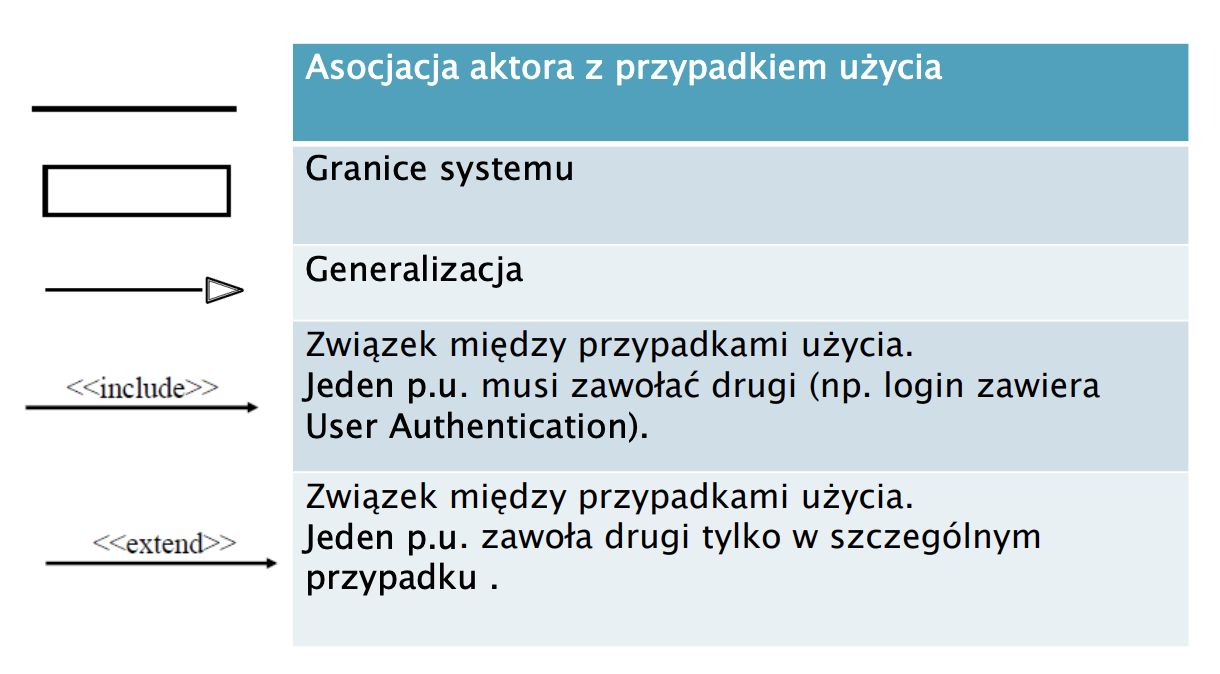
\includegraphics[width=\linewidth]{usecases.png}
\end{figure}

\section{Wprowadzenie do UMLa - część druga}

\subsection{Diagram klas}
    \begin{itemize}
        \item przedstawia strukturę systemu w modelach obiektowych przez ilustrację
        struktury klas i zależności między nimi,
        \item przedstawia podział odpowiedzialności pomiędzy klasy systemu i
        rodzaj wymienianych pomiędzy nimi komunikatów,
        \item jeden z najczęściej używanych, zwłaszcza do generowania kodu.
    \end{itemize}

\textbf{Klasy} służą do opanowania słownictwa tworzonego systemu. Mogą obejmować pojęcia związane z dziedziną danego
problemu, a także z jego implementacją. Używa się ich
do przedstawienia bytów programowych, sprzętowych,
koncepcyjnych.
\begin{itemize}
    \item simple names - $Customer$
    \item path names - $Bussiness_Rules::FraudAgent$
\end{itemize}

\begin{figure}[!h]
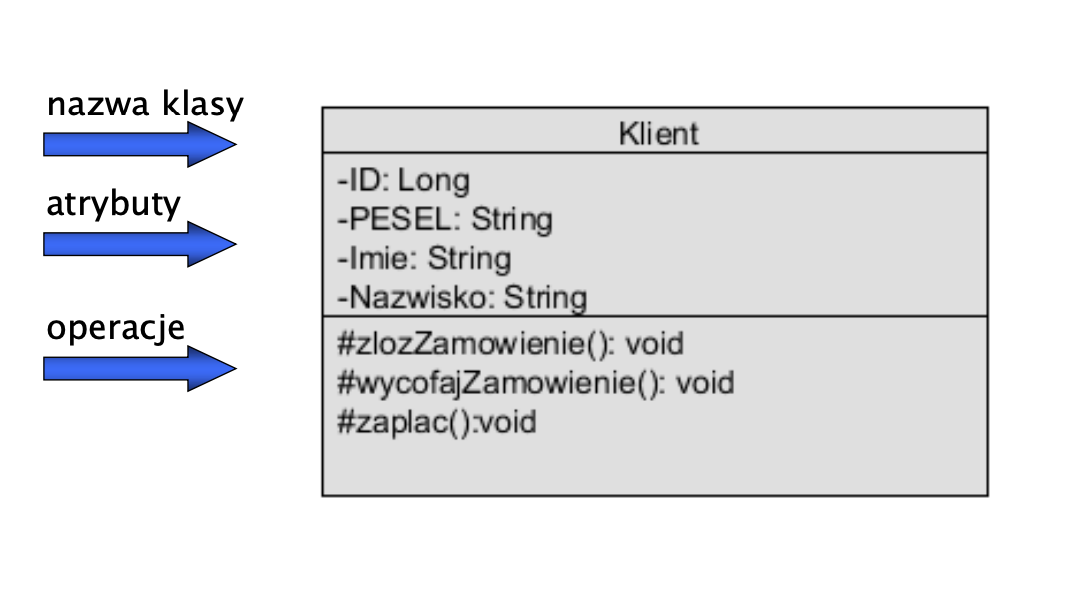
\includegraphics[width=\linewidth]{diagram_klasy.png}
\end{figure}

    \begin{itemize}
        \item \textbf{Parametr} - zawartość obiektu.
        \item \textbf{Atrybut} - nazwana właściwość klasy. Można dokładniej określić przez podane jego
        klasy i domyślnej wartości początkowej.
        \item \textbf{Operacja} (metoda) - implementacja pewnej usługi, której wykonania można zarządać
        od każdego obiektu klasy. Dokładne określenie przez podanie sygnatury (typy i domyślne wartości parametrów)
        \item \textbf{Odpowiedzialność} - wyrażenie zobowiązań klasy (lista).\\

        \begin{itemize}
            \item $+$ - public
            \item \# - protected
            \item $-$ private
        \end{itemize}
        \item instance - każdy egzemplarz przechowuje oddzielną wartość
        \item classifier - jest tylko jedna wartość wspólna dla wszystkich egzemplarzy
        \item ilość wystąpień - liczba w prawym górnym rogu ($1 = singleton$)
    \end{itemize}

    \textbf{Związki pomiędzy klasami}
    \begin{itemize}
        \item Zależność - strzałka przerywana,
        \item Asocjacja  - linia ciągła,
        \item Agregacja (częściowa) - linia
ciągła zakończona pustym rombem,
        \item Agregacja całkowita/zawieranie/kompozycja - linia ciągła zakończona pełnym
rombem
        \item Dziedziczenie - linia ciągła zakończona
        pustą strzałką.
        \item Implementacja - linia przerywana
        zakończona pustą strzałką.
        \\
        \item Rozszerzenia
        \begin{itemize}
            \item stereotypy - służą do stworzenia nowego
rodzaju obiektu ma podstawie innego obiektu
będącego już w standardzie UML.
            \item ograniczenia - dotyczą zarówno klas jak i
związków między nimi.
        \end{itemize}
    \end{itemize}

    \textbf{Szablony} - klasy parametryzowane. Parametry szablony w prostokącie z przerywanych linii
    obok diagramu klasy.

\subsection{Procesy wytwarzania oprogramowania}
    Proces tworzenia oprogramowania to
\textbf{zbiór czynności} i związanych z nimi
wyników, \textbf{prowadzących do powstania
systemu} informatycznego - tworzenie oprogramowania od zera,
rozszerzanie i modyfikowanie istniejących systemów.

Można wyróżnić cztery fundamentalne działania wspólne dla wszystkich procesów:
    \begin{itemize}
        \item Specyfikowanie oprogramowania
        \begin{itemize}
            \item zebranie wymagań,
            \item definiowanie funkcjonalności i ograniczeń dotyczących
tworzonego software’u.
        \end{itemize}
        \item Tworzenie oprogramowania (zgodnego ze specyfikacją)
        \item Walidacja oprogramowania
        \item Ewolucja oprogramowania (by ciągle zaspokajało zmieniające się potrzeby użytkownika)
    \end{itemize}


\textbf{Cykl życia systemu} obejmuje cały okres istnienia systemu, czyli
    \begin{itemize}
        \item studium zastosowalności
        \item analizę i specyfikację,
        \item projektowanie i tworzenie
        \item wdrażanie,
        \item pielęgnację,
        \item aspekty usprawnienia
    \end{itemize}

\subsection{Modele procesu wytwarzania oprogramowania}
\textbf{Model cyklu życia} systemu informatycznego ma na celu przedstawienie procesu wytwarzania
    oprogramowania, który prowadzi do stworzenia działającego systemu.


\subsubsection{Model kaskadowy}
\begin{itemize}
    \item podzielone na wyizolowane etapy, każdy musi być zakończony przed rozpoczęciem kolejnego
    \begin{itemize}
        \item Planowanie - cele biznesowe, podstawowe wymagania, założenia, standardy, parametry
        \item Analiza - zdefiniowanie przeznaczenia systemu $\rightarrow$ kompletny, spójny i jednoznaczny model systemu
        \item Projekt - dekompozycja na podsystemy, wybór strategii budowania, projektowanie obiektów, wybór komponentów, opis interfejsów
        \item Implementacja - tworzenie kodu źródłowego, mapowanie modeli na kod
        \item Testowanie - znajdowanie różnic między rzeczywistym elementem a jego modelem
        \item Pielęgnacja
    \end{itemize}
    \item Każdy etap podzielony na dwie części: twórczą i weryfikacji
    \item Ponowna praca, jeśli konieczna, jest wykonywana w kolejnych etapach - bardzo wysoki ksozt błędów
    popełnionych we wstępnych etapach.
    \item Koszty opracowania i akceptacji dokumentów są wysokie, zatem iteracje też - powinien bvyć używany
    tylko jeśli wymagania są jasne i zrozumiałe, adaptowanie zmian baredzo kosztowne.
    \item Marginalizacja roli klienta w procesie wytwarzania oprogramowania. Uzyskanie produktu zgodnego z wymaganiami
    silnie zależna od ich stabilności.
\end{itemize}

\subsubsection{Model V}
\begin{figure}[!h]
    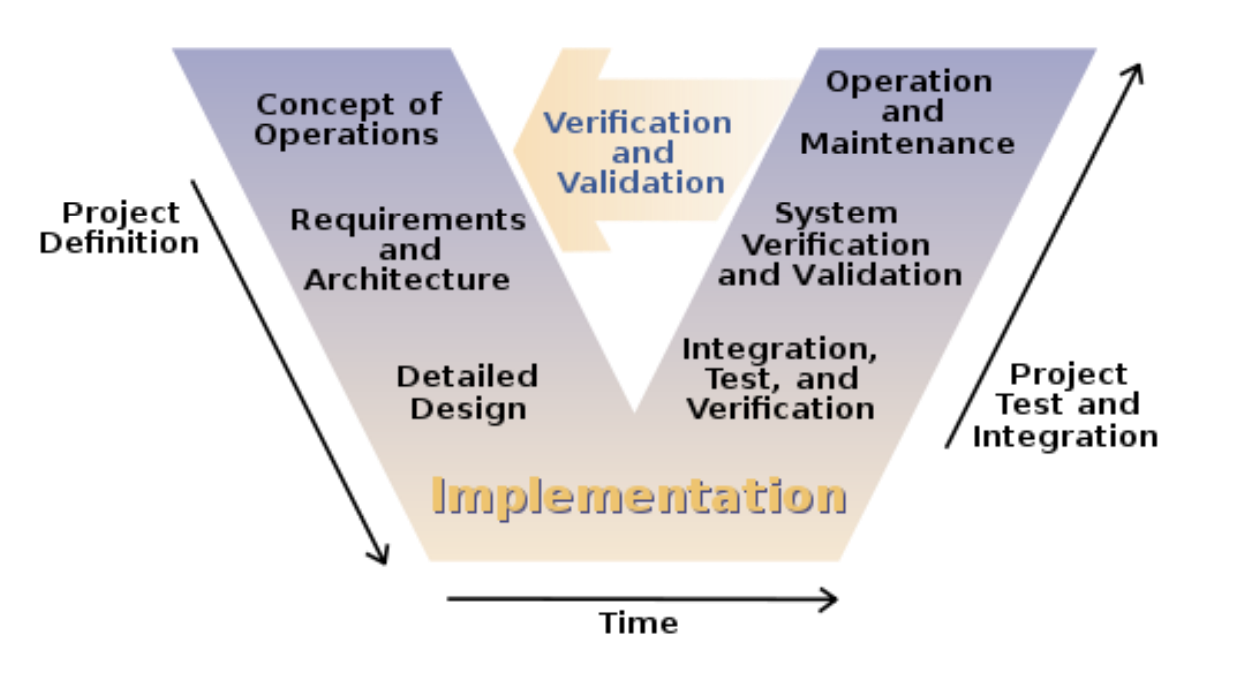
\includegraphics[width=\linewidth]{model_v.png}
\end{figure}

\subsubsection{Model Ewolucyjny}
\begin{figure}[!h]
    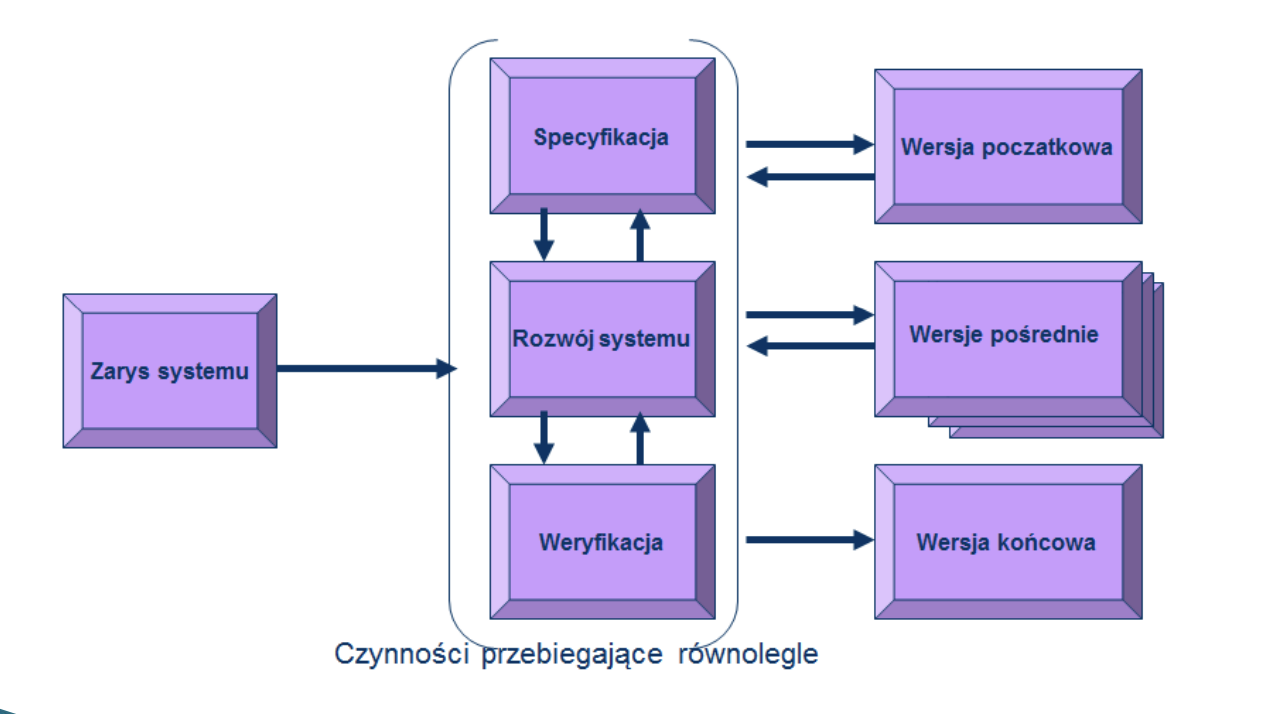
\includegraphics[width=\linewidth]{model_ewolucyjny.png}
\end{figure}
    \begin{itemize}
        \item pozwala później określić wymagania do projektowanego
systemu;
        \item prototyp pomaga kształcić przyszłego użytkownika;
        \item prototyp podnosi koszty w krótszej perspektywie, ale w
dłuższej może je obniżać
        \item zwykle prototyp jest wyrzucany;
    \end{itemize}

\subsubsection{Model iteracyjny}
\begin{figure}[!h]
    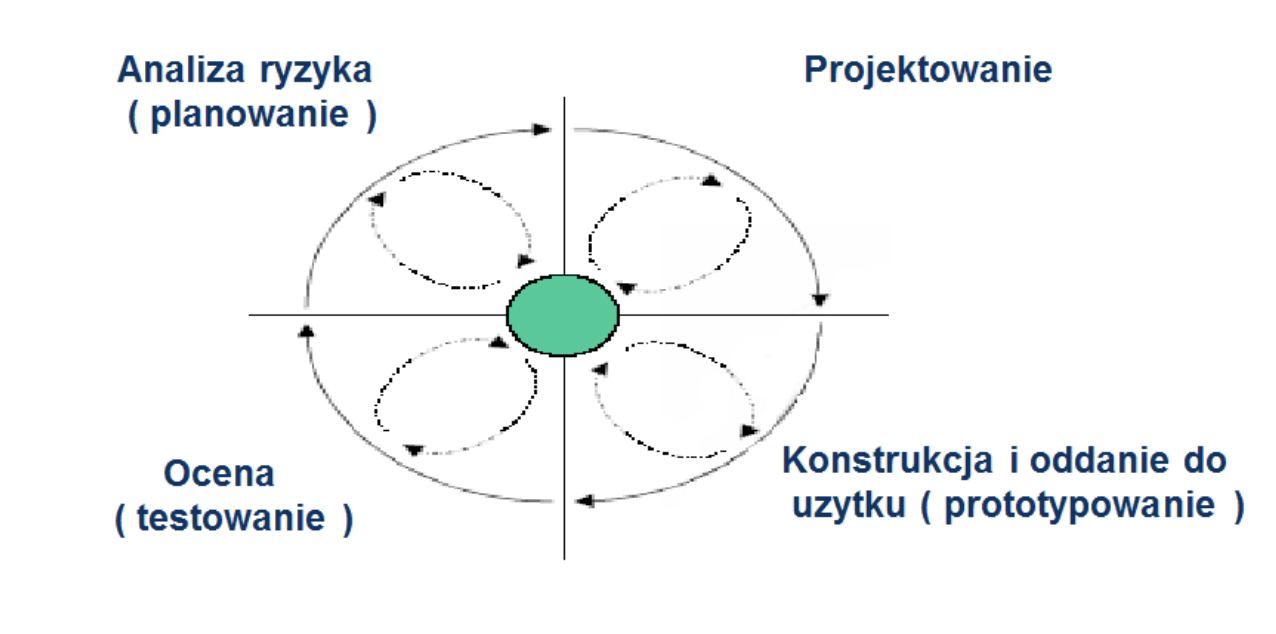
\includegraphics[width=\linewidth]{model_iteracyjny.png}
\end{figure}
    \begin{itemize}
        \item pozwala na wczesne wykrywanie błędów;
        \item łączy iteracje z klasycznym modelem kaskadowym;
        \item łatwość wprowadzania zmian;
        \item wymogi klienta dotyczące harmonogramu mogą utrudnić korzystanie z tego
         modelu;
        \item problemy z oszacowaniem ryzyka.
    \end{itemize}

\subsubsection{Model spiralny}
\begin{figure}[!h]
    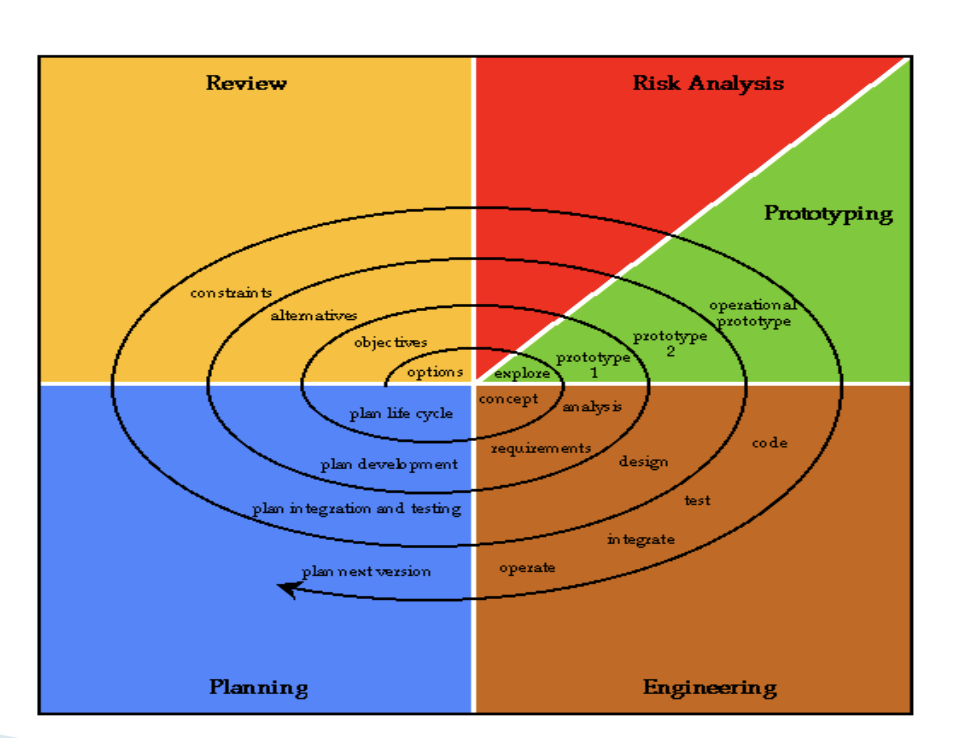
\includegraphics[width=\linewidth]{model_spiralny.png}
    Cechy modelu spiralnego:
    \begin{itemize}
        \item ciągłe monitorowanie i pomiar zmian;
        \item zmiany poddawane są review użytkownika;
        \item próba minimalizacji ryzyka niepowodzenia;
    \end{itemize}
\end{figure}

\section{Standardy jakości}

Syndrom LOOP - Late, Over budget, Overtime, Poor quality.

Mimnusy takiego podejścia:
\begin{itemize}
    \item Ważniejszy proces niż samo oprogramowanie
    \item Tworzenie ton dokumentacji
    \item Spora cześć procesu jest
    fikcyjna
    \item Dyscyplina zabija
    inicjatywę!
\end{itemize}

\subsection{CMM - Capability Maturity Model}
    Przeznaczony do oceny procesu wytwórczego służacego do produkcji oprogramowania.
    Ocenia praktyki stosowane podczas produkcji.
Model ocenia proces w skali pięciostopniowej, od chaotycznego (nic nie jest
sterowane ani kontrolowane),  aż do ścisłego,
zdyscyplinowanego procesu uwzględniającego wszystkie potrzebne aspekty.

    Model CMM obejmuje pięć aspektów:
    \begin{itemize}
        \item Poziomy dojrzałości
        \item Kluczowe obszary procesowe
        \item Cele
        \item Atrybuty procesu
        \item Kluczowe praktywki
    \end{itemize}

    Wyróżnia się pięć poziomów dojrzałości:
    \begin{itemize}
        \item POZIOM 1 - WSTĘPNY
        \begin{itemize}
            \item Procesy mające działania ad hoc (tymczasowe, doraźne).
            \item Organizacja bez stabilnej technologii wytwarzania i utrzymywania produktów.
            \item Zakres projektów realizowanych zupełnie nieprzewidywalny.
        \end{itemize}
        \item POZIOM 2 - POWATARZALNY
        \begin{itemize}
            \item Proces posiada dokumentowane standardy dokumentacji, szkoleń, utrzymywania stworzonego oprogramowania.
            \item Projekt ma w miarę ustabilizowane środowisko pracy i procedury zarządzania.
        \end{itemize}
        \item POZIOM 3 - ZDEFINIOWANY
        \begin{itemize}
            \item Pojawia się spójny zbiór definicji i standardów ukonstytuowany
            nie tylko na poziomie projektu, ale również na poziomie
            organizacji realizującej projekt.
            \item W zespole wyodrębniają się specjaliści od realizacji
            poszczególnych zadań, a organizacja dąży do wyposażenia ich
            w niezbędną wiedzę i umiejętności.
            \item Organizacja zaczyna na podstawie własnych doświadczeń
            modyfikować sposób prowadzenia projektów, tak aby
            maksymalnie odpowiadał specyfice organizacji i tworzonego
            przez nią produktu.
        \end{itemize}
        \item POZIOM 4 - ZARZĄDZANY
        \begin{itemize}
            \item Jeżeli proces jest zarządzany to znaczy, że w jakimś
zdefiniowanym obszarze wyniki podejmowanych działań
przenoszą określone rezultaty, które można zmierzyć za
pomocą wcześniej zdefiniowanych metryk.
            \item Zadania, których wykonanie nie generuje dużej liczby
błędów mogą być kontrolowane z mniejszą
częstotliwością, zaś obszary zdefiniowane jako
potencjalnie niebezpieczne np. w związku ze zmianą
technologii, mogą podlegać ściślejszej kontroli.
        \end{itemize}
        \item POZIOM 5 - OPTYMALIZUJĄCY
        \begin{itemize}
            \item Proces jest już tak dobrze zorganizowany i zarządzany, że
            nie pozostaje nic innego, jak tylko dalsze podnoszenie
            stawianych przed procesem wymagań.
            \item Celem stawianym na tym poziomie jest optymalizacja i
            dalsze ulepszanie procesu, zwiększanie jego
            efektywności (polepszanie wyników) oraz wydajności
            (zmniejszanie kosztów).
        \end{itemize}
    \end{itemize}


\subsection{ISO 9000}
Jeden z najbardziej znanych standardów dotyczących jakości. Wymaga, aby firma udokumentowała wszystkie swoje procedury związane z wytwarzaniem oprogramowania.

\begin{figure}[!h]
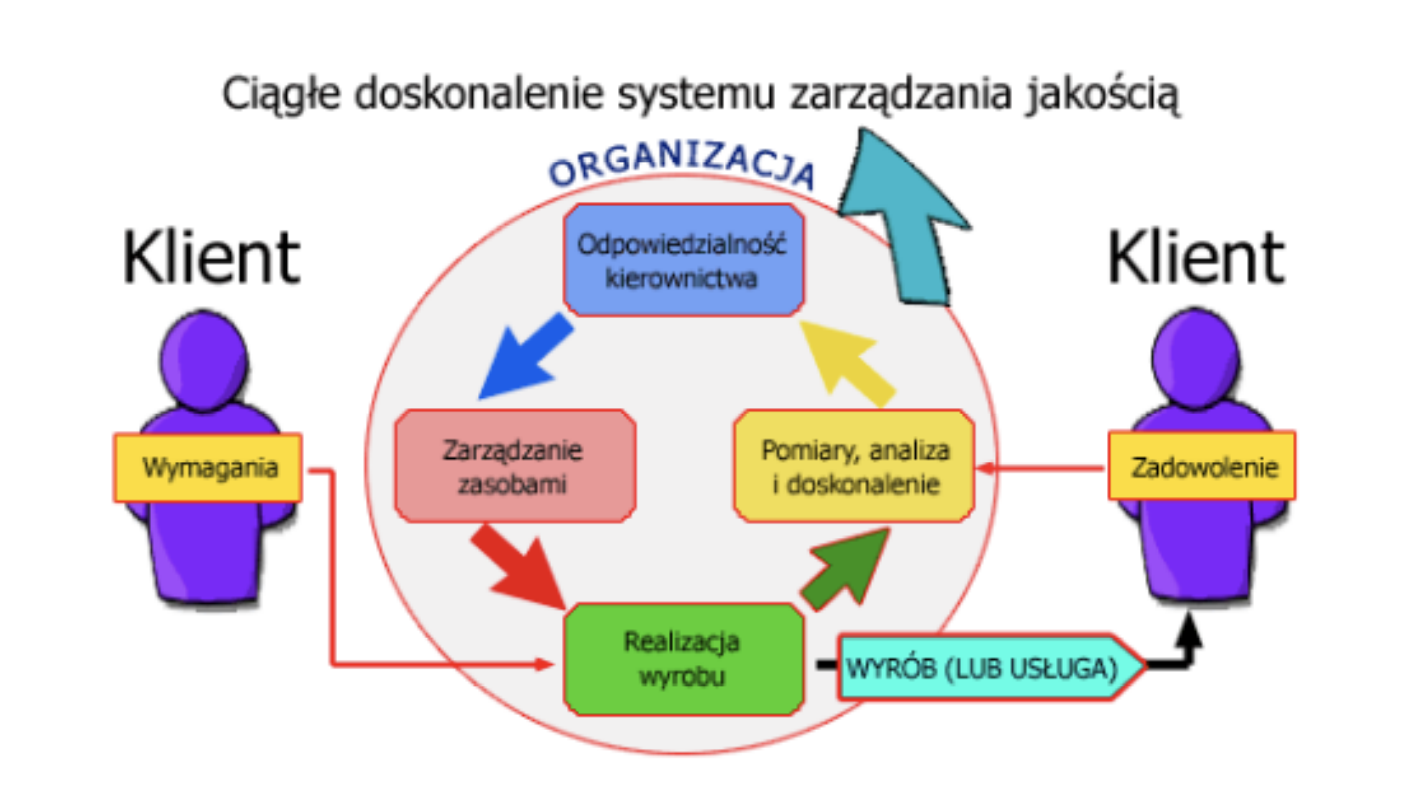
\includegraphics[width=\linewidth]{model_ISO.png}
\end{figure}

\begin{itemize}
    \item Odpowiedzialność kierownictwa
    \begin{itemize}
        \item Kierownictwo organizacji odpowiada za
        właściwe jej funkcjonowanie.
        \item Ustala misję i politykę organizacji,
        następnie określa odpowiednie cele do
        osiągnięcia.
        \item Do realizacji tych celów opracowuje plan
        działań i przyznaje odpowiednie zasoby
        do ich realizacji.
    \end{itemize}
    \item Zarządzanie zasobami
    \begin{itemize}
        \item Jest to zespół procesów
        związanych z zasobami jakie
        występują w organizacji.
        \item Te zasoby to ludzie (zasoby
        ludzkie), infrastruktura oraz
        środowisko pracy.
    \end{itemize}
    \item Realizacja wyrobu
    \begin{itemize}
    \item To zespół procesów bezpośrednio związany z
    realizacją wyrobu lub usługi.
    \item Wejściem są wymagania klienta, a wyjściem jest
    dostarczony wyrób lub usługa.
    \end{itemize}
    \item Pomiary, analiza i doskonalenie
    \begin{itemize}
        \item Procesy w organizacji i zadowolenie klienta
        wymagają systematycznego monitoringu, analizy i
        podejmowania działań doskonalących, aby wiedzieć
        jak postrzega nas klient (zadowolenie) oraz jak
        funkcjonują procesy w organizacji (zielona strzałka).
    \end{itemize}
    \item Ciągłe doskonalenie
    \begin{itemize}
        \item Ciągłe doskonalenie systemu zarządzania jakością
        możemy rozumieć jako ciągłe zwiększanie
        skuteczności i efektywności w realizacji polityki,
        strategii i celów organizacji.
    \end{itemize}
\end{itemize}

\section{Zwinne procesy wytwarzabua oprogramowania}
Manifesto for Agile Software Development
\begin{itemize}
    \item Individuals and interactions $\rightarrow$ Teamwork and responsibility
    \item Working software $\rightarrow$ Business value
    \item Customer collaboration $\rightarrow$ Partnership elaboration
    \item Respodning to change $\rightarrow$ Prepare for change
\end{itemize}
Lightweight (XP, Scrum) or fuller (DSDM, AUP) approaches.

\subsection{Programowanie ekstremalne - XP}
\begin{figure}[!h]
    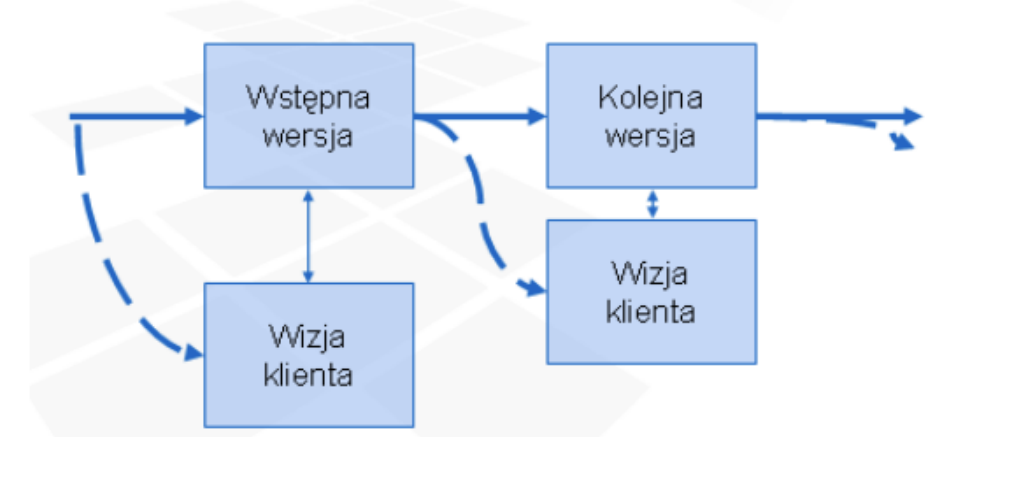
\includegraphics[width=\linewidth]{model_xp.png}
\end{figure}

Projekt informatyczny jest szczelnym systemem 4 zmiennych: daty dostarczenia, kosztu, liczby
defektów oraz niekompletności funkcji. Stawia na współpracę zespołu z klientem. Zakłada, że klient w dowolnym momencie może
zmienić zdanie i zaproponować zmianę wymagań.
Wady:
\begin{itemize}
    \item brak fazy projektowania i dokumentacji;
    \item krótka perspektywa planowania;
    \item silne założenie, ze klient pracuje cały czas z
zespołem;
\end{itemize}

Wartości:
    \begin{itemize}
        \item Komunikacja - przede wszystkim werbalna.
        \item Prostota - rozpoczynamy od najprostszego rozwiązania, spełniającego
wymagania; refaktoryzacja pozwala na adaptacje oprogramowania do
zmian.
        \item Sprzężenie zwrotne - obejmuje kilka aspektów (system, klient, zespół).
        \item Odwaga - potrzebna by: od razu produkować kod; refaktoryzować; wyrzucić zbędny kod.
        \item Szacunek - do pracy i czasu innych; między członkami zespołu.
    \end{itemize}

Struktura zespołu:
    \begin{itemize}
        \item Role podstawowe: programiści, klient
        \item Role pomocnicze: tester, coach, tracker
    \end{itemize}

User Stories:
    \begin{itemize}
        \item opisują funkcje systemu z punktu widzenia użytkownika
        \item ważne by miały wartość dla klienta,
        \item powinny być testowane
    \end{itemize}

Gra planistyczna:
    \begin{itemize}
        \item pisanie user story (klient)
        \item oszacowanie user story (informatycy)
        \item dziele user story/wybór zakresu iteracji (klient)
    \end{itemize}

Zapewnianie jakości:
    \begin{itemize}
        \item prostota;
        \item unikanie optymalizacji;
        \item TDD (Test Driven Development);
        \item automatyczne testowanie;
        \item refaktoryzacja.
    \end{itemize}

Testy akceptacyjne:
    \begin{itemize}
        \item pochodzą od klienta (w ten sposób dokładnie określa
        zachowanie systemu);
        \item najlepiej gdy mogą być wykonywane automatycznie (tester);
    \end{itemize}

Programowanie parami:
    \begin{itemize}
        \item zaleca się, by całość kodu pisana była w parach;
        \item częste zmiany w parach;
        \item wspólny standard kodowania;
        \item kod jest własnością całego zespołu;
        \item niezbędny system kontroli wersji.
    \end{itemize}

\begin{figure}
    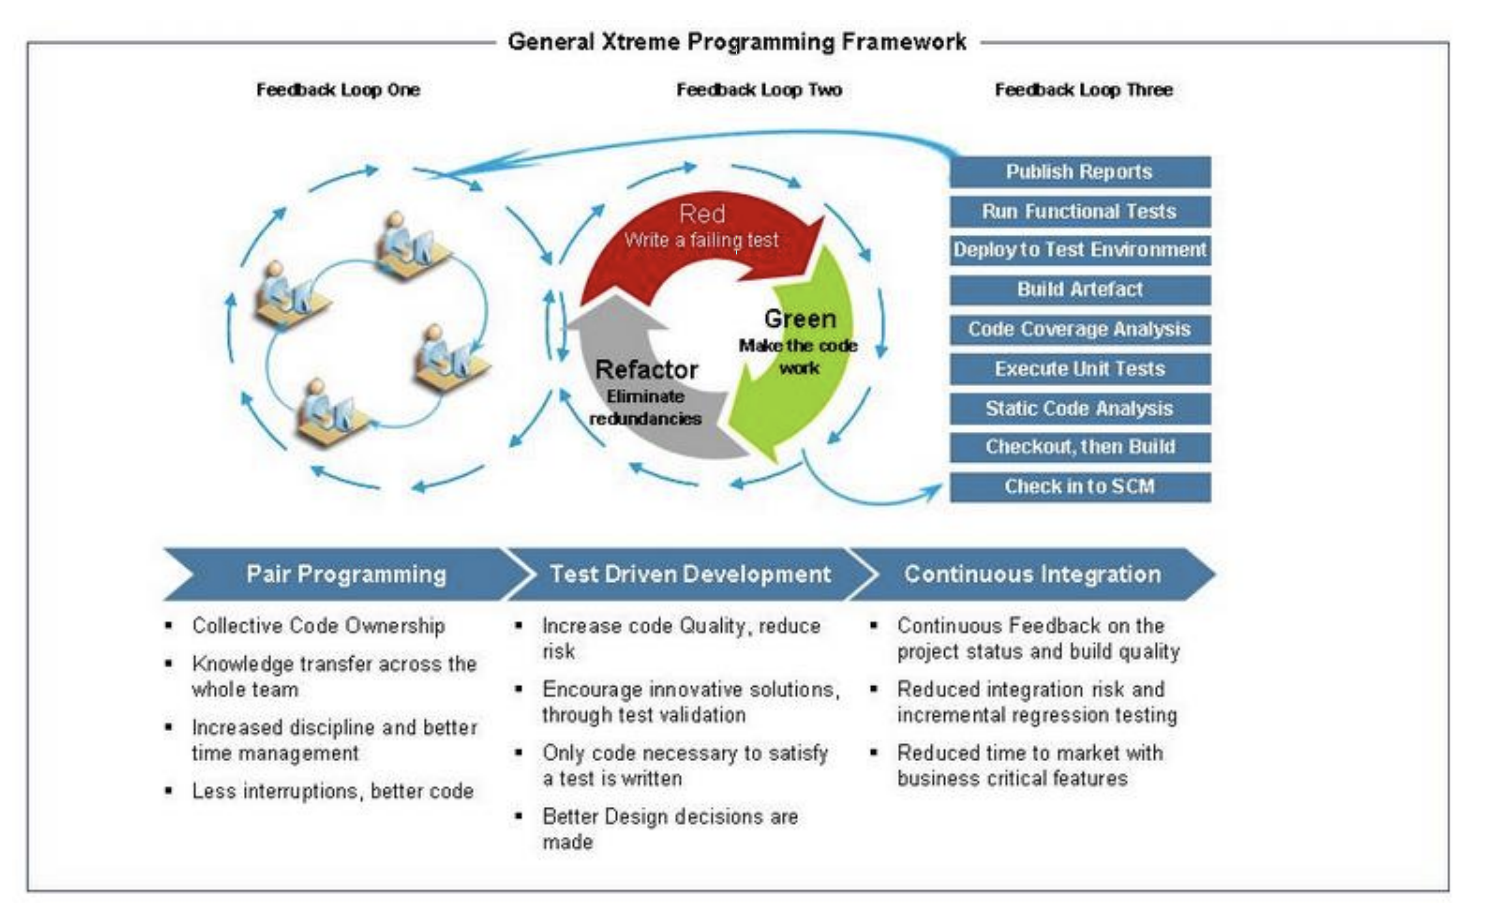
\includegraphics[width=\linewidth]{xp_framework.png}
\end{figure}

\subsection{SCRUM}
Metoda przy użyciu której ludzie mogą z powodzeniem rozwiązywać złożone problemy
adaptacyjne, by w sposób produktywny i kreatywny wytwarzać produkty o najwyższej możliwej wartości.
\begin{itemize}
    \item lekki;
    \item łatwy do zrozumienia;
    \item bardzo trudny do opanowania.
\end{itemize}

Trzy filary teorii SCRUMa:
\begin{itemize}
    \item Adaptacja - powinna być ciągła. Korekta musi być
wykonana jak najszybciej, by ograniczyć dalsze
następstwa problemów.
    \item Przejrzystość - wszystkie istotne aspekty procesu
muszą być widoczne dla osób odpowiedzialnych
za osiągane rezultaty.
    \item Inspekcja - – poddawane regularnej inspekcji są
zarówno scrumowe artefakty jak i postępy prac.
\end{itemize}



Scrum przewiduje cztery formalne punkty
przeprowadzania inspekcji i okazje do dokonania
korekty (adaptacji) - zdarzenia.
\begin{itemize}
    \item Planowanie Sprintu Sprint PlanningMeeting)
    \item Codzienny Scrum (Daily Scrum)
    \item Przegląd Sprintu (Sprint Review Meeting)
    \item Retrospektywa Sprintu (Sprint Retrospective)
\end{itemize}

W obręb Scruma wchodzą Zespoły Scrumowe
(Scrum Teams) oraz związane z nimi: role,
zdarzenia, artefakty i reguły postępowania.

\begin{tabular}{|c|c|c|}
\hline
ROLES & ARTIFACTS & EVENTS\\
\hline
Product Owner & Increment & Sprint\\
Development Team & Product Backlog & Sprint Planning\\
Scrum Master & Sprint Backlog & Daily Scrum\\
& & Sprint Review\\
& & Retrospective\\
\hline
\end{tabular}

Role w SCRUMie:
\begin{itemize}
    \item Właściciel Produktu (Product Owner) jest odpowiedzialny za
maksymalizację wartości produktu i pracy Zespołu
Deweloperskiego. Właściciel Produktu jest jedyną osobą zarządzającą
Rejestrem Produktu (Product Backlog) co
rozumiemy przez:
    \begin{itemize}
        \item jasne artykułowanie elementów Rejestru Produktu i określanie
ich kolejności w sposób zapewniający osiąganie założonych
celów i misji;
        \item zapewnianie, że Rejestr Produktu jest dostępny, przejrzysty
oraz jasny dla wszystkich i, że dobrze opisuje to, czym
Zespół Scrumowy będzie się zajmował.
    \end{itemize}
    \item Zespoł deweloperski:
    \begin{itemize}
        \item jest złożony z profesjonalistów;
        \item ma za zadanie dostarczenie (na zakończenie
każdego Sprintu), gotowego do wydania
Przyrostu produktu;
        \item zalecana liczebność: 3-9 osób;
        \item są samoorganizujące się.
        \item jest wielofunkcyjny, w swoim składzie posiadają
wszystkie umiejętności niezbędne do
wytworzenia Przyrostu;
        \item Scrum nie przewiduje tytułów innych niż
„Deweloper” dla członków Zespołu
Deweloperskiego;
        \item odpowiedzialność za wykonywaną pracę ponosi
cały Zespół Deweloperski; nie składają się z
podzespołów.
    \end{itemize}
    \item Scrum Master jest odpowiedzialny za to, by Scrum był rozumiany i
stosowany. Scrum Masterzy dokonują tego poprzez upewnianie się, że
Zespół Scrumowy stosuje się do założeń teorii Scruma, jego praktyk i reguł postępowania.
Scrum Master wspiera zarówno Właściciela Produktu jak i zespól deweloperski.
\end{itemize}

Zdarzenia w SCRUMie:
\begin{itemize}
    \item używane do wprowadzenia regularności;
    \item są ograniczone czasowo;
    \item każde (oprócz Sprintu) jest okazją do inspekcji i adaptacji.
    \\
    \item SPRINT – serce Scruma
    \begin{itemize}
        \item ograniczenie czasowe trwające jeden miesiąc lub krócej;
        \item Podczas Sprintu wytwarzany jest Przyrost „Ukończonej”,
używalnej i potencjalnie gotowej do wydania funkcjonalności;
        \item ma stałą długość przez cały okres trwania prac;
        \item niedozwolone są zmiany, które wpłyną na cel Sprintu;
        \item skład Zespołu Deweloperskiego i jego cel jakościowy
pozostają niezmienne.
    \end{itemize}
    \item Przerwanie Sprintu
    \begin{itemize}
        \item tylko Właściciel Produktu ma prawo to zrobić;
        \item Sprint może zostać przerwany, jeśli cel Sprintu się
zdezaktualizuje;
        \item powinien zostać przerwany, jeśli kontynuowanie prac nie ma
sensu w zaistniałych okolicznościach;
        \item przerwania Sprintów zużywają zasoby, ponieważ wszyscy
muszą się przegrupować podczas kolejnego Planowania
Sprintu, aby móc rozpocząć nowy Sprint.
    \end{itemize}
    \item Planowanie Sprintu:
    \begin{itemize}
        \item Jest ograniczone czasowo (8h dla miesięcznego
sprintu i proporcjonalnie);
        \item Część pierwsza: Co będzie zrobione w tym Sprincie?\\
Wejście:
\begin{itemize}
    \item Rejestr Produktu;
    \item ostatni przyrost;
    \item przewidywana pojemność ZD;
    \item ostatnie odczyty wydajności;
\end{itemize}
Wyjście:
\begin{itemize}
    \item elementu Rejestru Produktu
wybrane do zaimplementowania;
    \item Cel Sprintu.
\end{itemize}
        \item Część druga: Jak wybrana praca będzie wykonana?\\
Zespół deweloperski zwykle rozpoczyna od stworzenia projektu
systemu i planu prac niezbędnych do przetworzenia
elementów Rejestru Produktu w działający Przyrost produktu.
Zanim Planowanie Sprintu dobiegnie końca, Zespół
Deweloperski powinien móc wytłumaczyć Właścicielowi
Produktu i Scrum Masterowi, w jaki sposób ma zamiar
pracować, organizując się samodzielnie, by osiągnąć Cel
Sprintu i wytworzyć oczekiwany Przyrost.
    \end{itemize}
    \item Codzienny Scrum jest spotkaniem ograniczonym
czasowo do 15 minut, w którym każdy z
członków zespołu wyjaśnia:
    \begin{itemize}
        \item Co zostało wykonane od ostatniego potkania?
        \item Co zostanie wykonane przed kolejnym spotkaniem?
        \item Jakie przeszkody stoją na drodze?
    \end{itemize}
    \item Przegląd Sprintu organizowany jest na zakończenie
Sprintu w celu przeprowadzenia inspekcji
Przyrostu i dostosowaniu, jeśli zajdzie taka
potrzeba, Rejestru Produktu.
Podczas Przeglądu Sprintu Zespół Scrumowy i
interesariusze wspólnie omawiają to, co zostało
ukończone w Sprincie.
Może trwać maksymalnie 4h dla miesięcznego
Sprintu.
Przegląd Sprintu obejmuje następujące punkty:
    \begin{itemize}
        \item Właściciel Produktu stwierdza, które funkcjonalności zostały
„Ukończone”, a które nie;
        \item Zespół Deweloperski omawia, co poszło dobrze w trakcie
Sprintu; jakie były problemy i jak je rozwiązano;
        \item Zespół Deweloperski prezentuje „Ukończoną” pracę i
odpowiada na pytania dotyczące Przyrostu,
        \item Właściciel Produktu omawia Rejestr Produktu w aktualnej
jego postaci. Przewiduje termin zakończenia prac.
        \item Cala grupa omawia kolejne kroki.
    \end{itemize}
    \item Retrospektywa Sprintu jest okazją dla zespołu
Scrumowego do przeprowadzenia inspekcji
swoich działań i opracowania planu usprawnień.
Ma na celu:
    \begin{itemize}
        \item Sprawdzenie, co działo się w ostatnim Sprincie, biorąc pod
uwagę ludzi, zależności, procesy i narzędzia;
        \item Zidentyfikowanie i uporządkowanie istotnych elementów, które
sprawdziły się w działaniu oraz tych, które kwalifikują się do
poprawy;
        \item Stworzenie planu wprowadzania w życie usprawnień sposobu
wykonywania pracy przez Zespół Scrumowy.
    \end{itemize}
\end{itemize}

Artefakty:
\begin{itemize}
    \item Rejestr Produktu to uporządkowana lista wszystkiego,
co może być potrzebne w produkcie oraz jedyne
źródło wymaganych zmian, które mają
wprowadzone.
Odpowiedzialny za RP jest Właściciel Produktu.
Elementy Rejestru Produktu posiadają następujące
atrybuty: opis, kolejność i oszacowanie (estymację).
    \item Rejestr Sprintu to podzbiór elementów Rejestru
Produktu wybranych do Sprintu rozszerzony o plan
dostarczenia Przyrostu produktu.
Rejestr Sprintu definiuje pracę, jaką Zespół
Deweloperski wykona by przekształcić elementy
Rejestru Produktu w „Ukończony” Przyrost.
Rejestr Sprintu jest dobrze widocznym, tworzonym w
czasie rzeczywistym obrazem pracy, jaką Zespół
Deweloperski planuje wykonać w trakcie Sprintu.
Rejestr Sprintu należy tylko i wyłącznie do Zespołu
Deweloperskiego.
    \\
    \item Monitorowanie postępów Sprintu – możliwe w
    każdym momencie Sprintu (Codzienny Scrum)
    \item Przyrost - suma wszystkich elementów Rejestru
    Produktu zakończonych podczas Sprintu i
    wszystkich Sprintów poprzednich. :
    Na koniec Sprintu nowy Przyrost musi być
    „Ukończony”.
    \item Aby zapewnić przejrzystość, wszyscy członkowie
danego zespołu muszą mieć wspólne
pojmowanie, co to znaczy, że praca jest
skończona. Pomaga w tym Definicja Ukończenia
dla Zespołu Scrumowego.
    \item W miarę jak Zespoły Scrumowe dojrzewają,
oczekuje się, że ich Definicja Ukończenia będzie
zawierała coraz bardziej rygorystyczne kryteria
zapewniania jeszcze wyższej jakości.
\end{itemize}

\subsection{AGILE PM (DSDM Atern)}
Fuller Approaches(but still agile)

\begin{figure}[!h]
    \includegraphics[width=\linewidth]{agile_principles.png}
\end{figure}

\begin{itemize}
    \item Focus on the business need
    \item Deliver on time
    \item Collaborate
    \item Never compromise quality
    \item Build incrementally from firm foundations
    \item Develop iteratively
    \item Communicate continuously and clearly
    \item Demonstrate control
\end{itemize}

\begin{figure}[!h]
    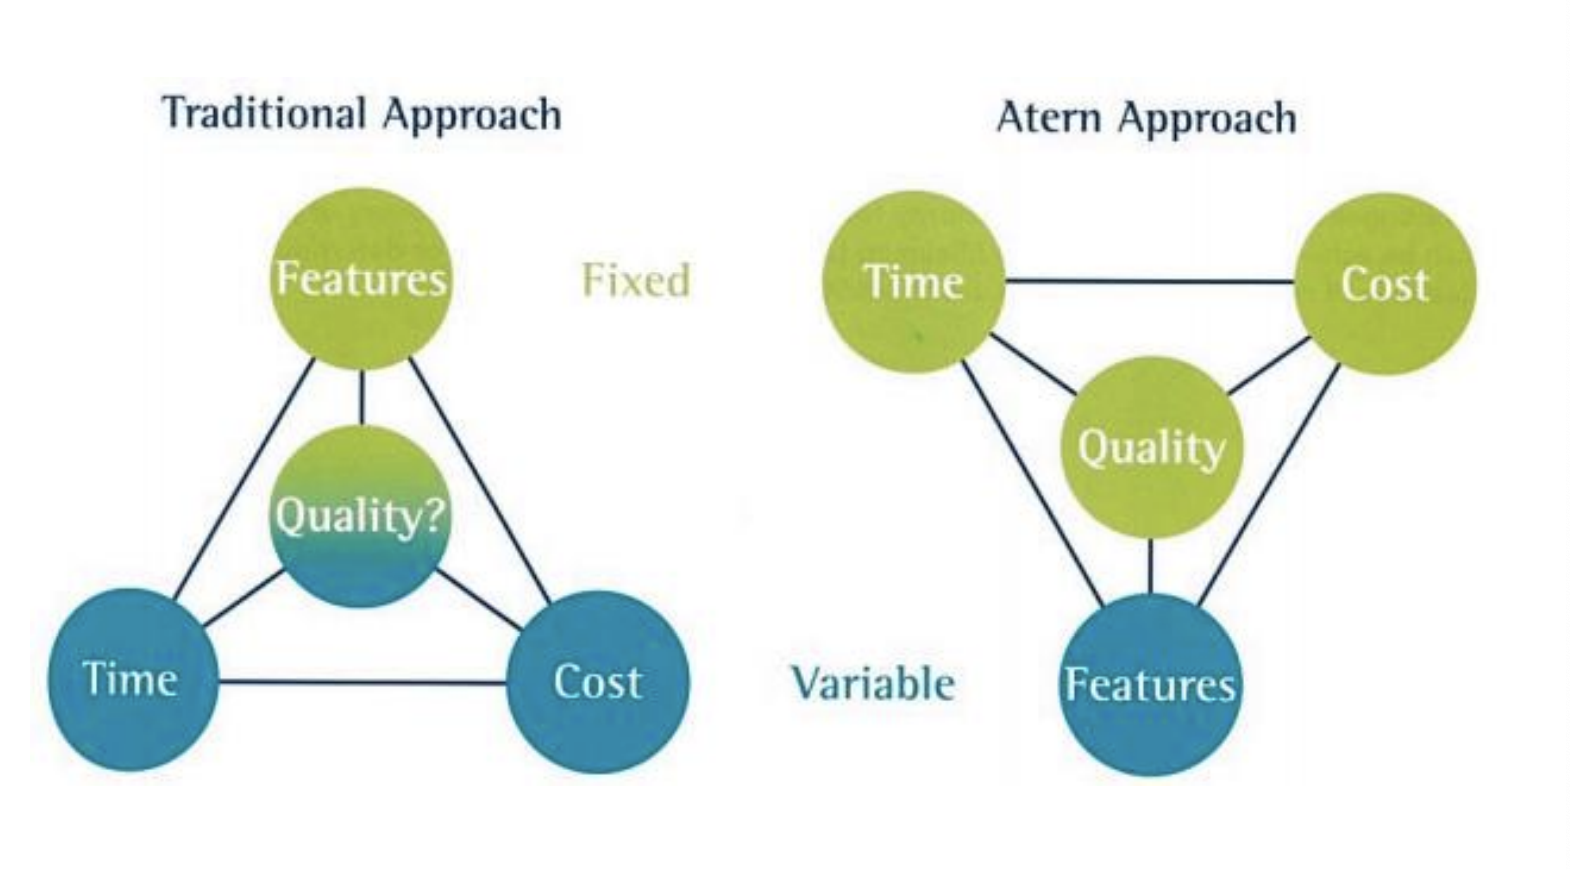
\includegraphics[width=\linewidth]{atern_approach.png}
\end{figure}

\subsubsection{Fazy projektu}
\begin{figure}[!h]
    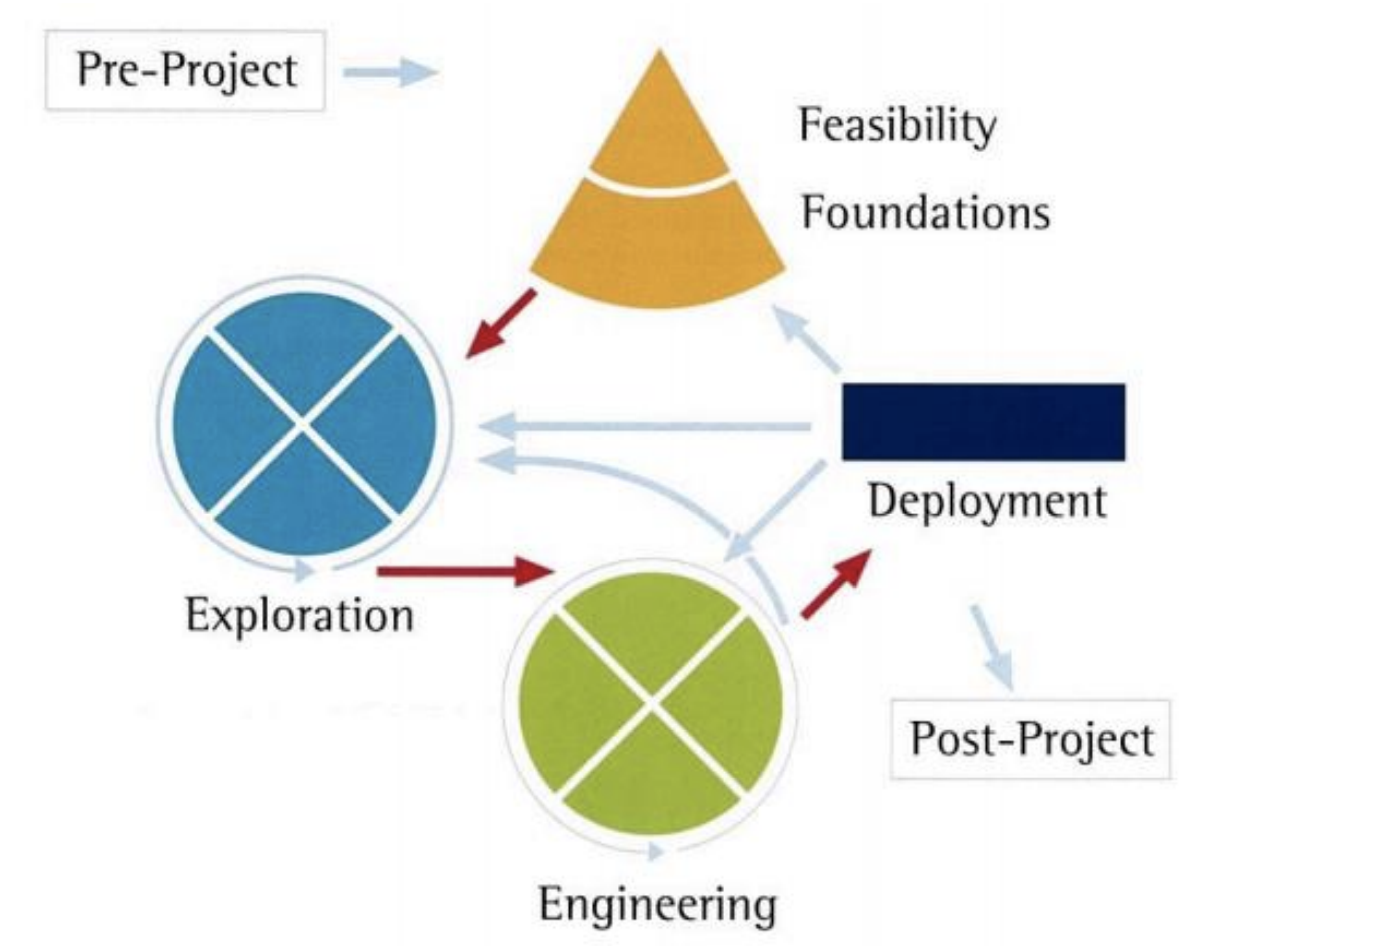
\includegraphics[width=\linewidth]{agile_fazy.png}
\end{figure}

\begin{itemize}
    \item PRE-PROJECT
    \begin{itemize}
        \item problem biznesowy, który będziemy rozwiązywać
        \item identyfikacja Business Sponsor i Business Visionary
        \item zakres, plan i zasoby na fazę Feasibility
    \end{itemize}
    \item FEASIBILITY
    \begin{itemize}
        \item ustalić wykonalność rozwiązania problemu biznesowego
        \item identyfikacja potencjalnych zysków
        \item zarys możliwych podejść do rozwiązania
        \item Pierwsze estymaty czasowe i kosztowe
    \end{itemize}
    \item FOUNDATIONS
    \begin{itemize}
        \item wysoko poziomowe wymagania
        \item identyfikacja wspieranych procesów biznesowych
        \item podstawy architektury systemu
        \item sposób zapewnienia wysokiej jakości
    \end{itemize}
    \item EXPLORATION
    \begin{itemize}
        \item uszczegóławianie wymagań
        \item pojawia się (iteracyjnie) działające rozwiązanie
        \item zarys możliwych podejść do rozwiązania
    \end{itemize}
    \item ENGINEERING
    \begin{itemize}
        \item rozwijanie rozwiązania z fazy Exploration
    \end{itemize}
    \item DEPLOYMENT
    \begin{itemize}
        \item potwierdzenie wydajności rozwiązania
        \item dostarczenie (iteracyjnie) rozwiązania
        \item dostarczenie potrzebnej dokumentacji
    \end{itemize}
\end{itemize}

\subsubsection{Role}
    DSDM Atern bardzo szczegółowo opisuje role i odpowiedzialności poszczególnych osób w projekcie.

    \begin{itemize}
        \item BUSINESS SPONSOR
        \begin{itemize}
            \item najwyższy rangą w projekcie
            \item jest właścicielem tzw. przypadku biznesowego
            \item zapewnia finansowanie i zasoby
        \end{itemize}
        \item BUSINESS VISIONARY
        \begin{itemize}
            \item definiuje wizję projektu i komunikuje ją
            \item ma zapewnić współprace na wszystkich poziomach projektu
            \item wkład w najważniejsze wymagania
            \item arbiter w przypadku sporów
        \end{itemize}
        \item PROJECT MANAGER
        \begin{itemize}
            \item monitoruje postęp projektu
            \item wysoko poziomowe planowanie harmonogramu
            \item zarządzanie ryzykiem w projekcie
            \item zatrudnia specjalistów
            \item Motywuje zespoły
        \end{itemize}
        \item TECHNICAL COORDINATOR
        \begin{itemize}
            \item definiuje środowisko pracy
            \item doradza w sprawach technicznych
            \item pilnuje standardów technicznych
            \item zajmuje się wymaganiami
niefunkcjonalnymi
        \end{itemize}
        \item TEAM LEADER
        \begin{itemize}
            \item skupiony na zespole
            \item pilnuje dostarczania poszczególnych komponentów na czas
            \item raportuje postęp do PM
            \item prowadzi spotkania zespołowe
        \end{itemize}
        \item BUSINESS AMBASSADOR
        \begin{itemize}
            \item rola biznesowa w zespole deweloperskim
            \item dzieli się perspektywa biznesową z zespołem
            \item dostarcza scenariusze biznesowe
            \item tworzy dokumentacje użytkownika
        \end{itemize}
        \item BUSINESS ANALYST
        \begin{itemize}
        \item komunikacja między biznesem a zespołem deweloperskim
        \item dystrybucja i wstępna akceptacja dokumentów biznesowych
        \end{itemize}
        \item SOLUTION DEVELOPER
        \begin{itemize}
            \item skupiony na dostarczeniu rozwiązania
            \item modele potrzebne do dostarczenia rozwiązania
            \item dokumentacja
        \end{itemize}
        \item SOLUTION TESTER
        \begin{itemize}
            \item definiuje scenariusze testowe, test casy
            \item komunikuje wyniki testów do TL
            \item pracuje z BAs nad testami akceptacyjnymi
        \end{itemize}
        \item
    \end{itemize}

\subsubsection{Produkty}

Levels of priority - \textbf{MoSCoW}
    \begin{itemize}
        \item \textbf{M}ust Have
        \item \textbf{S}hould Have
        \item \textbf{C}ould Have
        \item \textbf{W}on’t Have this time
    \end{itemize}

\begin{figure}[!h]
    \includegraphics[width=\linewidth]{agile_timebox.png}
\end{figure}
TIMEBOX jest podzielony na kilka faz.
    \begin{itemize}
        \item \textbf{Kick-off} – krótka sesja, która ma pomoc zrozumieniu celu timeboxa
        \item \textbf{Investigation} – szczegóły wszystkich produktów, które mamy wykonać
        \item \textbf{Refinement} – kodowanie i testowanie
        \item \textbf{Consolidation} – spinanie całości
    \end{itemize}


\begin{figure}[!h]
    \includegraphics{agile_iterative.png}
\end{figure}
Iterative development
\begin{itemize}
    \item \textbf{Identify}: zespół definiuje cel
    \item \textbf{Plan}: kto powinien zrobić co
    \item \textbf{Evolve}: wykonywanie
zaplanowanych czynności
    \item \textbf{Review}: sprawdzanie rezultatów
\end{itemize}


\begin{figure}[!h]
    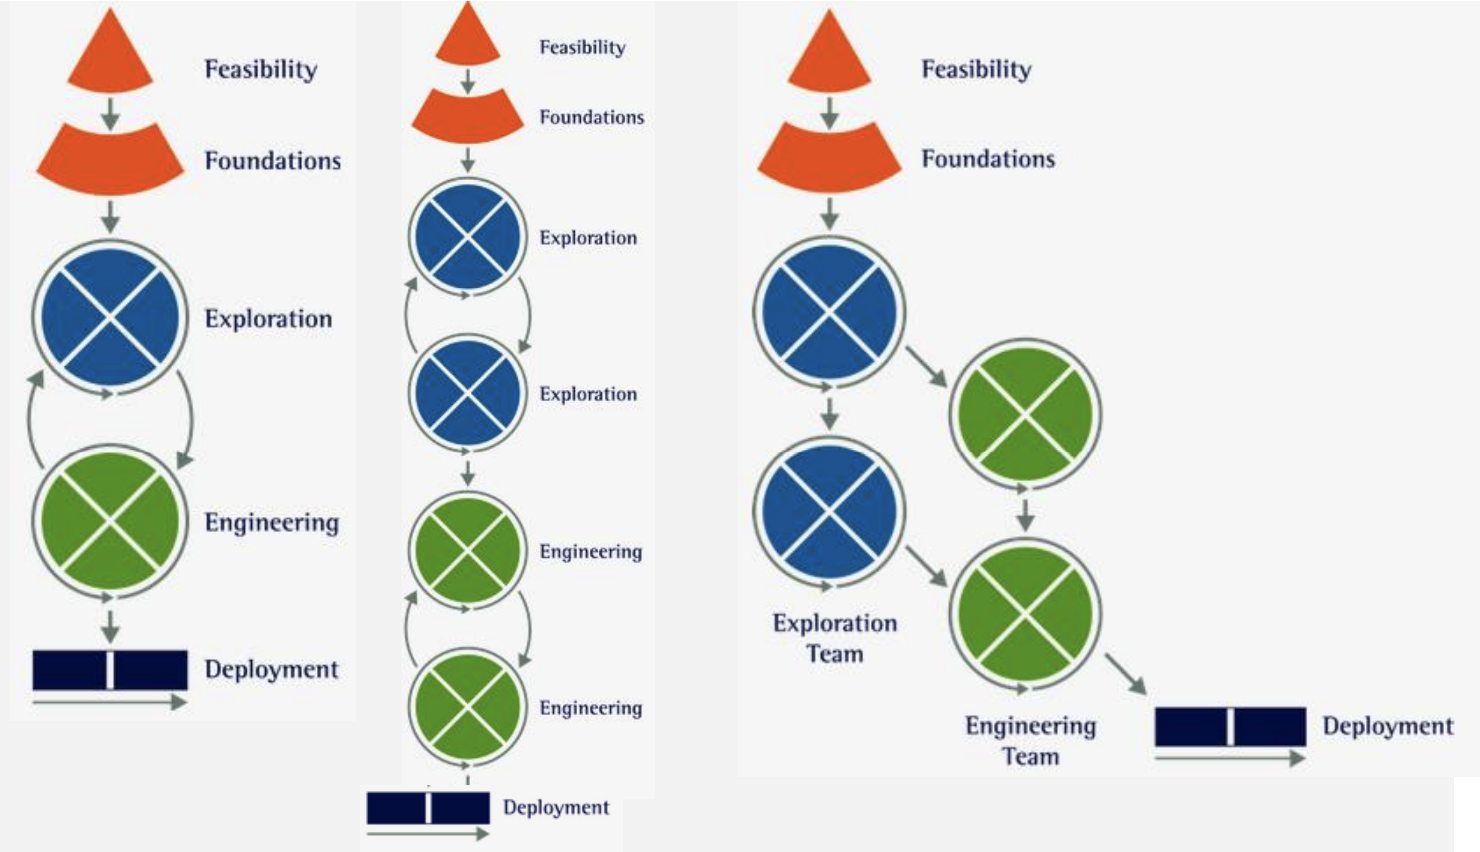
\includegraphics[width=\linewidth]{agile_iterations.png}
\end{figure}


\subsection{AUP - Agile Unified Process}

\begin{itemize}
    \item uproszczona wersja Rational Unified Process;
    \item stosuje zwinne techniki takie jak TDD, refactoring;
    \item twórcą jest Scott Ambler (2002r.)
    \item seryjny w dużej skali, iteracyjny w małej.
\end{itemize}


\begin{figure}[!h]
    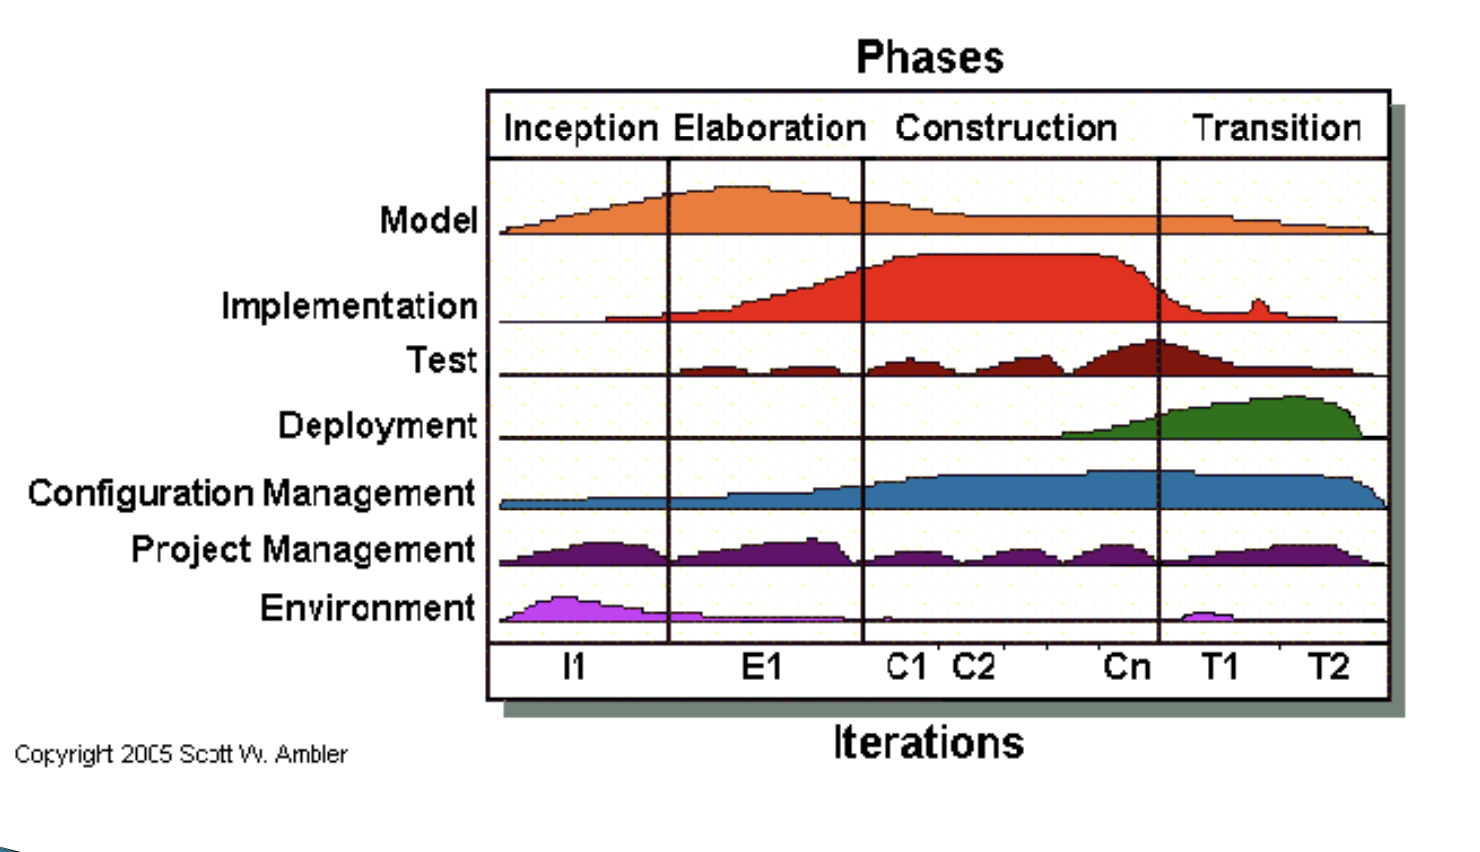
\includegraphics[width=\linewidth]{aup_phases.png}
\end{figure}


Zasady AUP
    \begin{itemize}
        \item twój zespół wie, co robi;
        \item prostota;
        \item zwinność;
        \item skupienie się na istotnych aktywnościach;
        \item niezależność od narzędzi;
        \item możliwość adaptacji.
    \end{itemize}


\subsection{KANBAN}
\begin{itemize}
    \item Kanban - jedna z podstaw systemów produkcyjnych
Toyoty (Toyota Production System) i pochodnych,
opartych o zasadę pull.
    \item System pull (w odróżnieniu od systemów push), sterowany
jest przez składane przez odbiorcę zamówienie, a
nie ogólny, arbitralny plan produkcji. Za pomocą
techniki kanban zapewnia się ciągły przepływ
produktu przez system produkcyjny.
    \item Pierwsze zastosowanie techniki kanban w IO - 2004 r.
w pracach Davida J. Andersona bazujących na
doświadczeniach zespołów wytwarzających
oprogramowanie w firmach Microsoft i Corbis.
    \item Chociaż proces wytwarzania oprogramowania znacząco
różni się od procesów przemysłowych, niektóre idee z
nich zaczerpnięte mogą być z powodzeniem stosowane.
W szczególności idea przepływu produktu przez
system, podczas którego systematycznie zwiększana
jest jego wartość, stoi u podstaw wszystkich metodyk
zwinnych (agile).
    \item Kanban odnosi się do etapowości procesu wytwarzania
oprogramowania (skojarzenia z procesami
kaskadowymi). Bez wątpienia jednak, nawet w
zespołach najpełniej stosujących podejście zwinne,
zawsze występują przynajmniej trzy stany pracy — do
zrobienia, w trakcie, gotowe.
\end{itemize}

Sześ reguł kanbana:
    \begin{itemize}
        \item odbiorca przetwarza dokładnie tyle elementów, ile opisane
jest na karcie kanban;
        \item dostawca wytwarza dokładnie tyle elementów, ile opisane jest
na karcie kanban;
        \item żaden element nie jest wytwarzany lub przekazywany
pomiędzy stanowiskami bez karty kanban;
        \item karta kanban musi towarzyszyć każdemu elementowi czy
półproduktowi przetwarzanemu w ramach systemu;
        \item elementy wadliwe lub występujące w niewłaściwych ilościach,
nigdy nie są przekazywane w dół procesu;
        \item limity obowiązujące na każdym z etapów (fizyczna ilość kart
kanban) są stopniowo obniżane aby redukować zapasy i
odkrywać nieefektywności procesów produkcji, dążąc do ich
doskonalenia.
    \end{itemize}

Kanban vs Scrum
\begin{figure}[!h]
    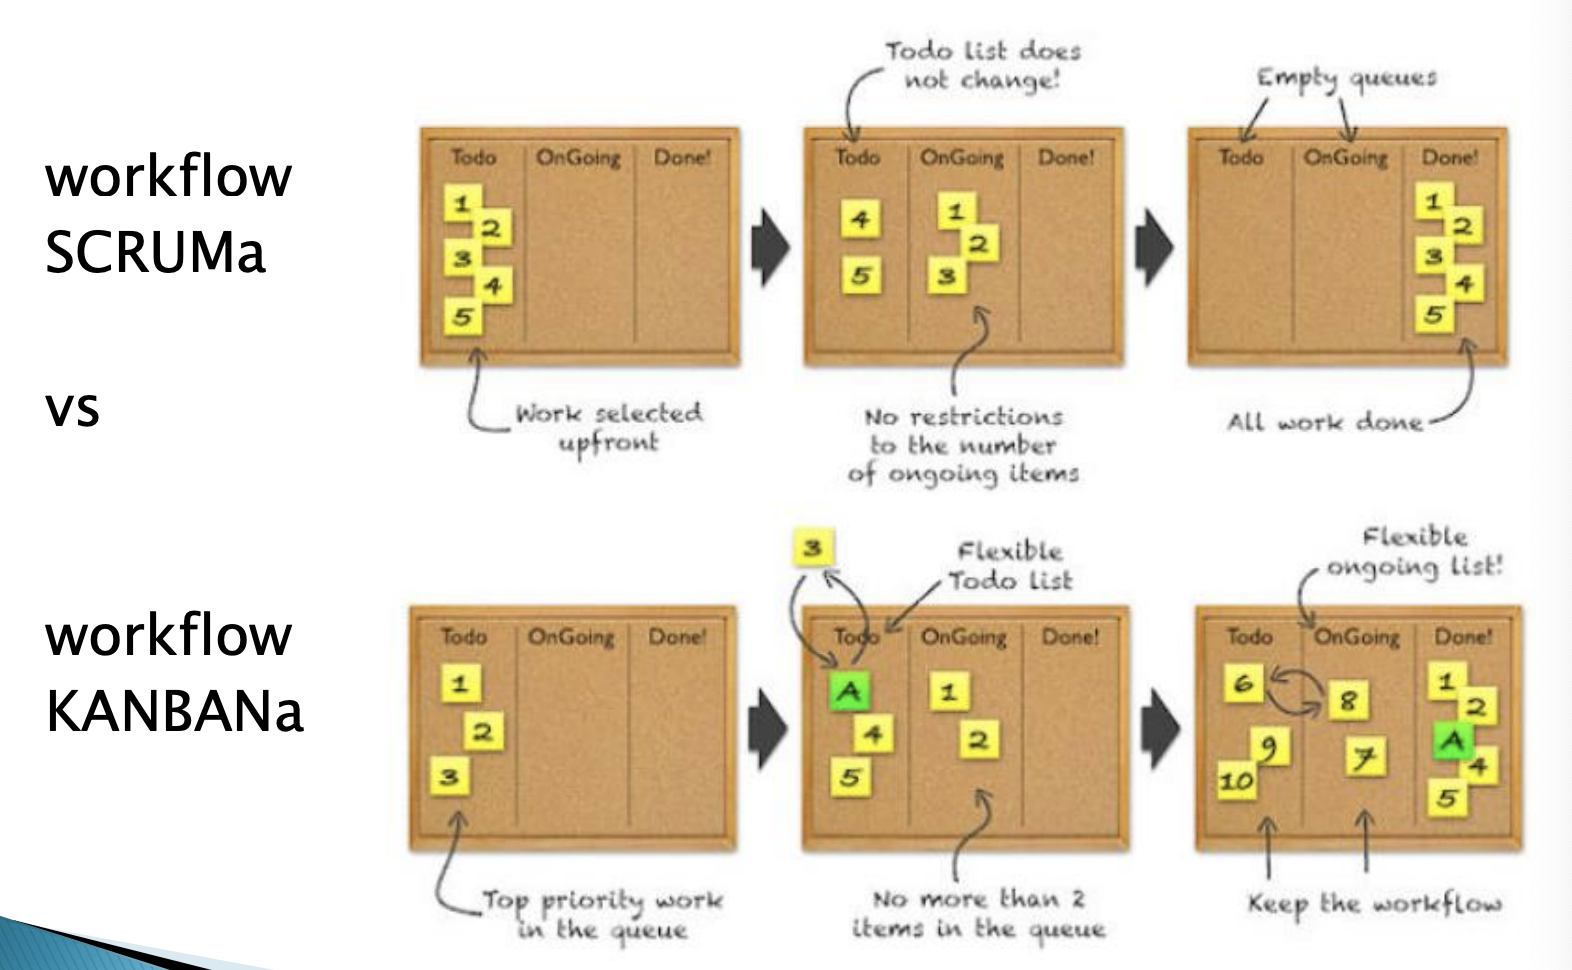
\includegraphics[width=\linewidth]{kanban_vs_scrum.png}
\end{figure}
\begin{figure}[!h]
    \includegraphics[width=\linewidth]{kanban_vs_scrum2.png}
\end{figure}
\begin{figure}[!h]
    \includegraphics[width=\linewidth]{kanban_vs_scrum3.png}
\end{figure}
\begin{figure}[!h]
    \includegraphics[width=\linewidth]{kanban_vs_scrum4.png}
\end{figure}

\begin{figure}[!h]
    \includegraphics[width=\linewidth]{kanban_vs_scrum5.png}
\end{figure}

\subsection{SCRUM-BAN}
SCRUM-BAN = SCRUM + KANBAN

\begin{figure}[!h]
    \includegraphics[width=\linewidth]{scrum_vs_scrumban.png}
\end{figure}


Kiedy używać Scrum-bana?
\begin{itemize}
    \item W projektach typu maintenance
    \item W projektach typu helpdesk
    \item W projektach z często dorzucanymi User stories
lub często zgłaszanymi bledami
\end{itemize}

\section{Wymagania}
\begin{itemize}
    \item Wymagania to opis funkcji (usług), które mają być
    realizowane przez system i opis ograniczeń dla systemu.
    \item Wymagania nie opisują jak system ma działać a co ma
    wykonywać.
    \item Wymagania są definiowane na wczesnych etapach
    rozwoju systemu jako specyfikacja tego, co ma być
    implementowane.
    \item W zakresie zarządzania projektem można wyróżnić
    różne typy wymagań stawianych systemowi.
    \item Inżynieria wymagań to proces pozyskiwania,
    analizowania, dokumentowania oraz weryfikowania
    wymagań dla projektowanego systemu.

\end{itemize}

\subsection{Klasyfikacja wymagań}
    Podział wymagań:
    \begin{itemize}
        \item Funkcjonalne:
        \begin{itemize}
            \item Wprowadzanie nowej faktury
            \item Generowanie raportu miesięcznego
        \end{itemize}
        \item Pozafunkcjonalne
        \begin{itemize}
            \item minimum 20 faktur na godzinę
            \item 200000h MTBF
            \item maksimum 2 godziny potrzebne na przeszkolenie
        1 pracownika
        \end{itemize}
    \end{itemize}

    Klasyfikacja wymagań - FURPS:
    \begin{itemize}
        \item Functionality – funkcjonalność
        \item Usability – użyteczność
        \item Reliability – niezawodność
        \item Performance – wydajność
        \item Security - bezpieczeństwo
    \end{itemize}


\subsubsection{Wymagania funkcjonalne}


„System powinien\dots”
Zalety:
\begin{itemize}
    \item łatwość spisywania;
\end{itemize}
Wady:
\begin{itemize}
    \item słaba czytelność;
    \item trudne sprawdzanie kompletności i spójności;
\end{itemize}

Funkcje systemu
Wady:
\begin{itemize}
\item słaba czytelność
\item trudne do zrozumienia
\end{itemize}

Przypadki użycia
Zalety:
\begin{itemize}
    \item łatwość spisywania;
    \item czytelność;
    \item łatwość zrozumienia i wyobrażenia sobie
przyszłego systemu;
\end{itemize}
Przypadek Użycia jest formą ustrukturalizowaną.

Historyjki użytkownika - Who? What? Why?
Cecha INVEST:
    \begin{itemize}
        \item Independent - Zależności powodują problem z estymacją.
        \item Negotiable.
        \item Valuable.
        \item Estimable.
        \item Small - zasada jednego sprinta.
        \item Testable.
\end{itemize}

\subsubsection{Wymagania pozafunkcjonalne}
Wymagania pozafunkcjonalne są to ograniczenia
usług lub funkcji udostępnianych przez
oprogramowanie, takich jak ograniczenia
czasowe, ograniczenia procesu rozwoju
oprogramowania, standardy, itp\dots

\begin{itemize}
    \item Niezawodność\\
Zbiór atrybutów opisujących zdolność
oprogramowania do spełnienia i utrzymania
określonych wymaga, co do jego stabilności
działania, przy spełnieniu określonych
warunków oraz w ścile określonych ramach
czasowych.\\
Atrybuty:
    \begin{itemize}
          \item Dojrzałość (ang. Maturity)
          \item Odporność na błędy (ang. Fault-tolerance)
          \item Zdolność do odtworzenia (ang. Recoverability)
    \end{itemize}
    \item Wydajność\\
Zbiór atrybutów opisujących powiązania miedzy
poziomem wydajności oprogramowania, a
wykorzystywanymi zasobami przy spełnieniu określonych
warunków.\\
Atrybuty:
    \begin{itemize}
        \item Wykorzystanie czasu
        \item Wykorzystanie zasobów
    \end{itemize}
    \item Użyteczność\\
Zbiór atrybutów opisujących nakład pracy
niezbędny do swobodnego posługiwania się
oprogramowaniem.\\
Atrybuty:
    \begin{itemize}
        \item Łatwość zrozumienia
        \item Łatwość nauki
        \item Operatywność
    \end{itemize}
    \item Łatwość konserwacji\\
Zbiór atrybutów opisujących nakład pracy
niezbędny do wprowadzenia zmian do
oprogramowania.\\
Atrybuty:
    \begin{itemize}
        \item Łatwość analizy (ang. Analysability)
        \item Łatwość wprowadzania zmian (ang. Changeability)
        \item Stabilność (ang. Stability)
        \item Łatwość testowania (ang. Testability)
    \end{itemize}
    \item Przenośność\\
Zbiór atrybutów opisujących zdolność
oprogramowania do przenoszenia między
różnymi środowiskami/platformami.\\
Atrybuty:
    \begin{itemize}
        \item Łatwość adaptacji (ang. Adaptability)
        \item Zgodność (ang. Conformance)
        \item Łatwość instalacji (ang. Installability)
        \item Łatwość zastąpienia (ang. Replaceability)
    \end{itemize}
\end{itemize}


Podsumowanie:
\begin{itemize}
    \item Wymagania pozafunkcjonalne stanowią niezbędne
uzupełnienie wymagan funkcjonalnych dla
oprogramowania;
\item Problemy z oprogramowaniem wskazuje na silną
potrzebę precyzyjnego definiowania atrybutów
(charakterystyk) dla tworzonych produktów
programistycznych;
\end{itemize}

\subsection{Analiza wymagań/analiza obiektowa}
\begin{itemize}
    \item Celem jest stworzenie modelu systemu, zwanego
modelem analitycznym.
    \item Wysiłek uczestników projektu skupia się na
strukturalizowaniu i formalizowaniu zabranych
wcześniej wymagań.
\end{itemize}

Definicje:
\begin{itemize}
    \item Model analityczny – reprezentuje tworzony system z
perspektywy użytkownika; opis co system powinien robić.
    \item Analityczny model obiektowy – odzwierciedla indywidualne
koncepcje korzystania z systemu, ich właściwości i relacje
między nimi (diagramy klas).
    \item Model dynamiczny - koncentruje się na zachowaniu systemu
(diagramy sekwencji i stanów).
    \item Obiekty encji – reprezentują trwałą informację potwarzaną
    przez system.
    \item Obiekty brzegowe – odzwierciedlają interakcje między
    aktorami a systemem.
    \item Obiekty sterujące – odpowiedzialne są za realizację
    przypadków użycia.
    \item Relacja dziedziczenia umożliwia hierarchiczne
    organizowanie koncepcji.
    \item Generalizowaniem nazywamy aktywność identyfikowania
    abstrakcyjnych koncepcji na podstawie przykładów i
    konkretyzacji.
    \item Specjalizowanie to aktywność odwrotna, czyli
    identyfikowanie koncepcji bardziej specyficznych na
    podstawie koncepcji wysokopoziomowej.
\end{itemize}

    \begin{figure}[h]
        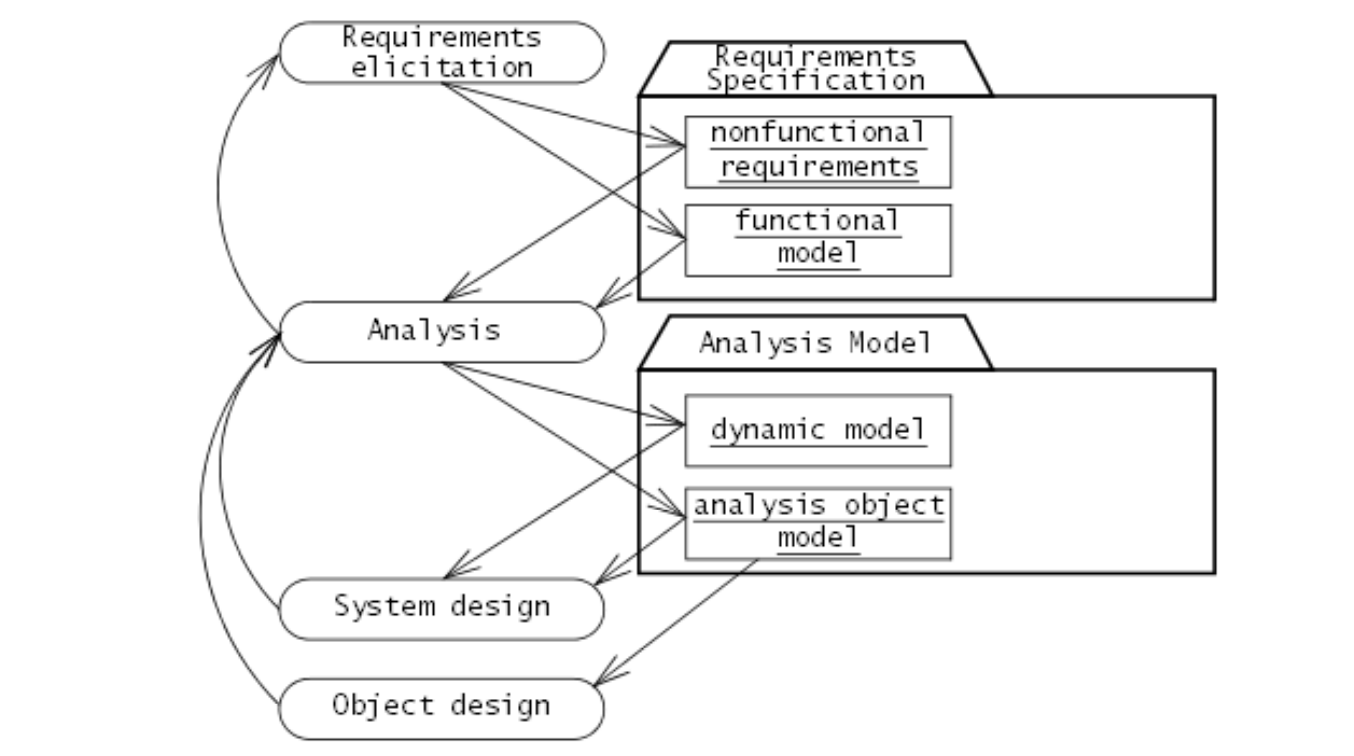
\includegraphics[width=\linewidth]{analiza_wymagan.png}
    \end{figure}

\section{Projektowanie systemu}
Projektowanie systemu to transformowanie
modelu analitycznego w model projektu systemu.

Projektowanie systemu można przedstawić w
postaci dekompozycji na następujące etapy:
\begin{itemize}
    \item rozpoznawanie celów projektowych
    \item projektowanie wstępnych dekompozycji
    \item doskonalenie dekompozycji stosownie do celów
projektowych
\end{itemize}

\begin{figure}[h]
    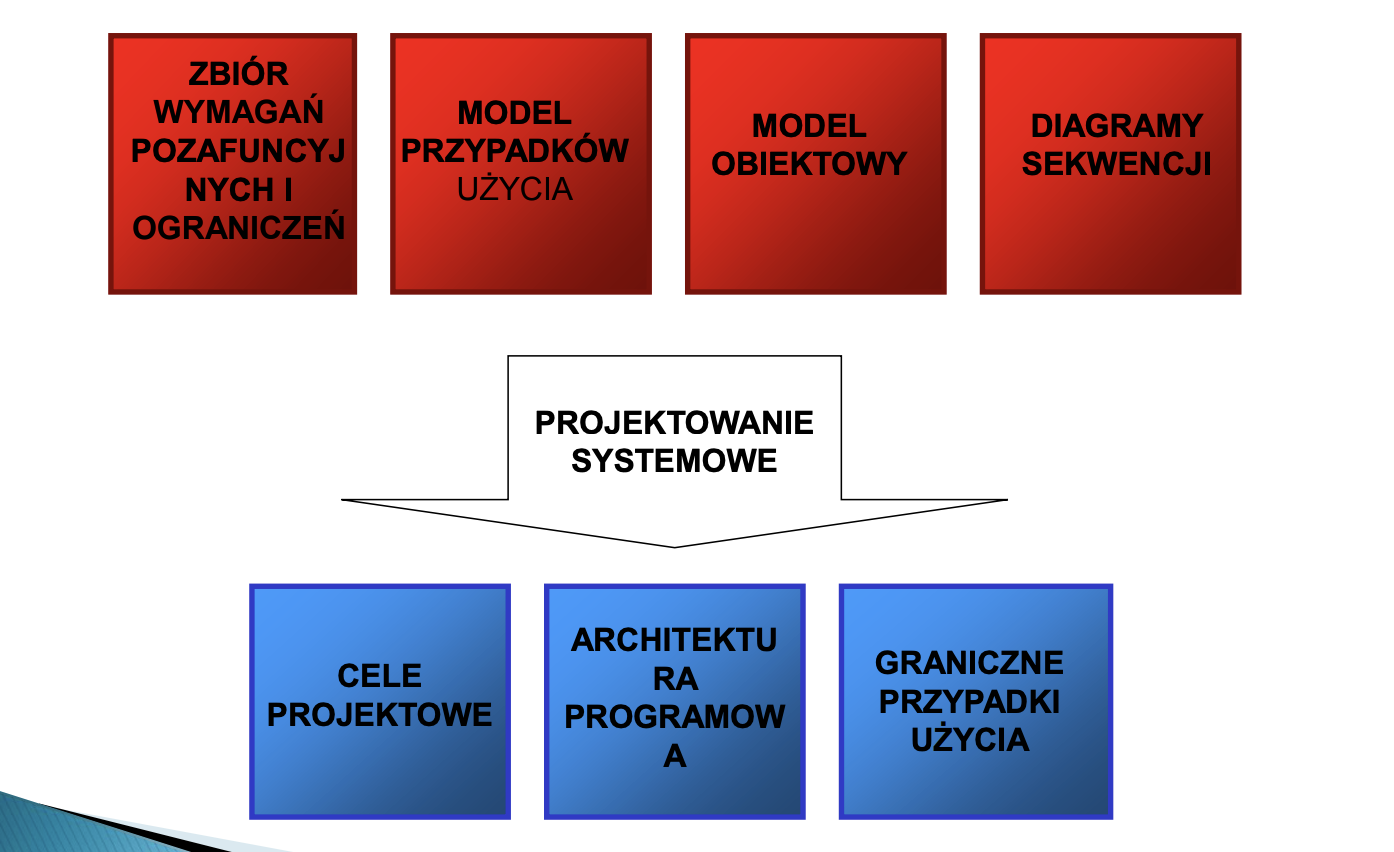
\includegraphics[width=\linewidth]{projekt_systemu.png}
\end{figure}

\subsection{Podstawowe pojęcia i koncepcje.}
\begin{itemize}
    \item Podsystem jest wymienną częścią systemu,
posiadającą dobrze zdefiniowane interfejsy i
hermetyzującą stan oraz zachowanie
składających się na nią klas. Rozróżniamy dwa główne typy komponentów:
logiczny i fizyczny.
    \item Usługa jest zbiorem powiązanych operacji
podporządkowanych realizacji wspólnego
celu. Projektowanie systemu skupia swe aktywności
na definiowaniu usług świadczonych przez
każdy podsystem.
    \item Sprzężeniem w zbiorze podsystemów nazywamy
stopień ich wzajemnego uzależnienia.
    \item Spoistość podsystemu jest miara uzależnienia jego
własnych klas.
    \item W trakcie projektowaniu systemu chcemy
zmaksymalizować jego spoistość i
zminimalizować sprzężenie.
    \item Efektem dekompozycji hierarchicznej jest
uporządkowany zbiór warstw. Warstwa stanowi
zgrupowanie podsystemów oferujących
powiązane usługi.
    \item Wyróżniamy dwa rodzaje architektury warstwowej:
otwartą i zamkniętą (np ISO/OSI, TCP/IP).
\end{itemize}


\subsection{Wzorce architektoniczne - poziom integracji komponentów}

\subsubsection{MVC: model-widok-kontroler}
Dzieli interaktywną aplikację na trzy części. Model zawiera korowa
funkcjonalność, którą następnie widoki wyświetlają. Kontroler obsługuje
żądanie użytkownika. Kontroler z widokami tworzą UI aplikacji.

    \begin{figure}[h]
        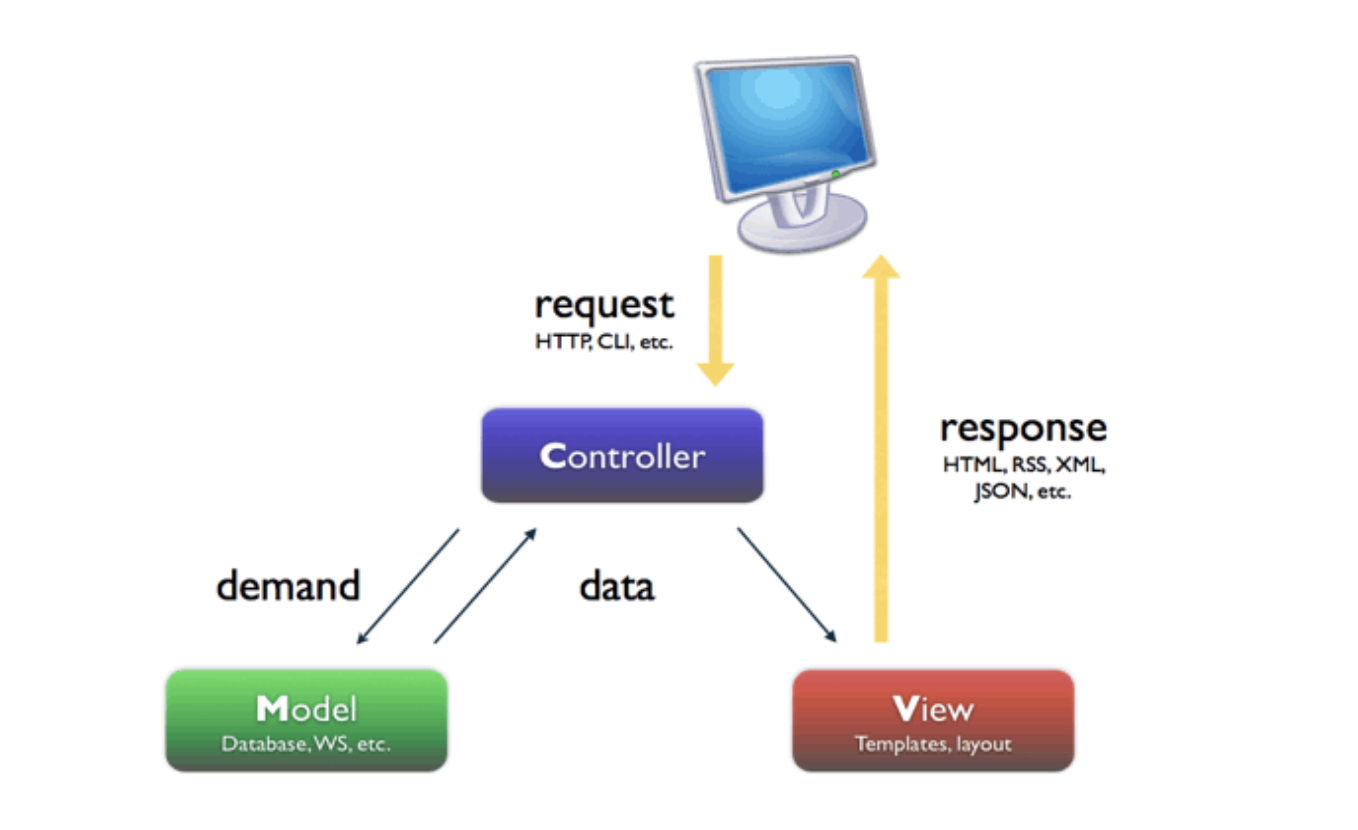
\includegraphics[width=.5\linewidth]{mvc.png}
        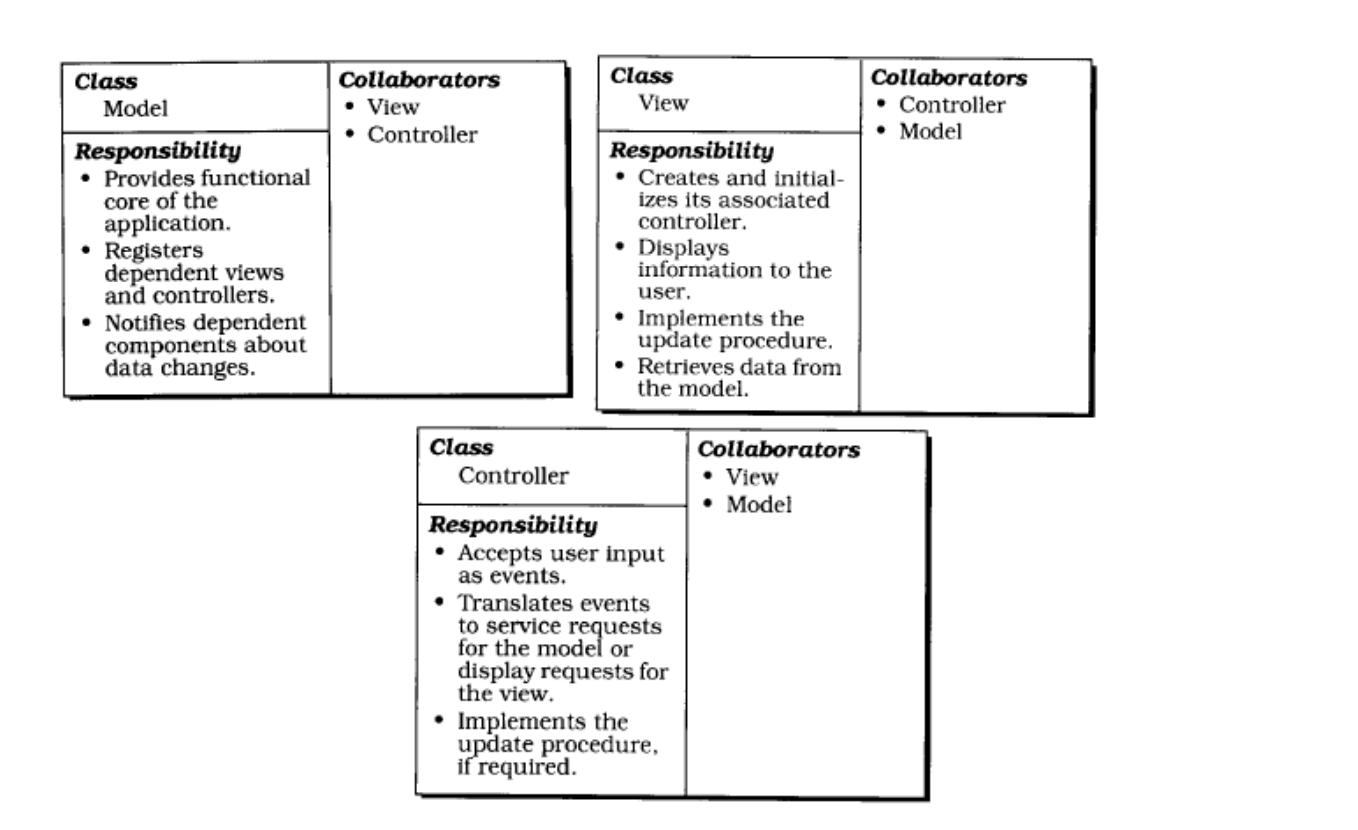
\includegraphics[width=.5\linewidth]{mvc-struktura.png}
    \end{figure}

Zastosowania: Smalltalk, Java/Swing.


\subsubsection{PAC: prezentacja-abstrakcja-kontrola}
Definiuje hierarchie kooperujących agentów, z których każdy
podzielony jest na trzy komponenty: prezentacji, abstrakcji kontroli.

\begin{figure}[h]
    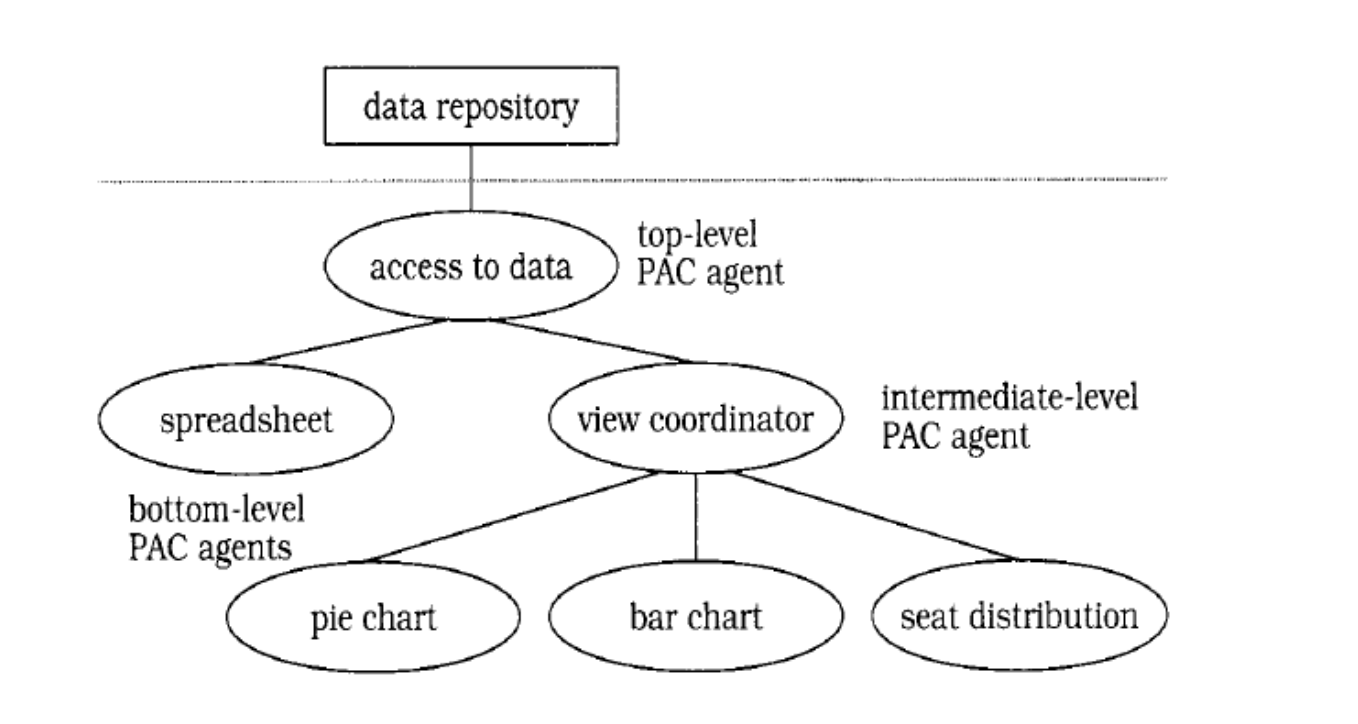
\includegraphics[width=.5\linewidth]{pac.png}
    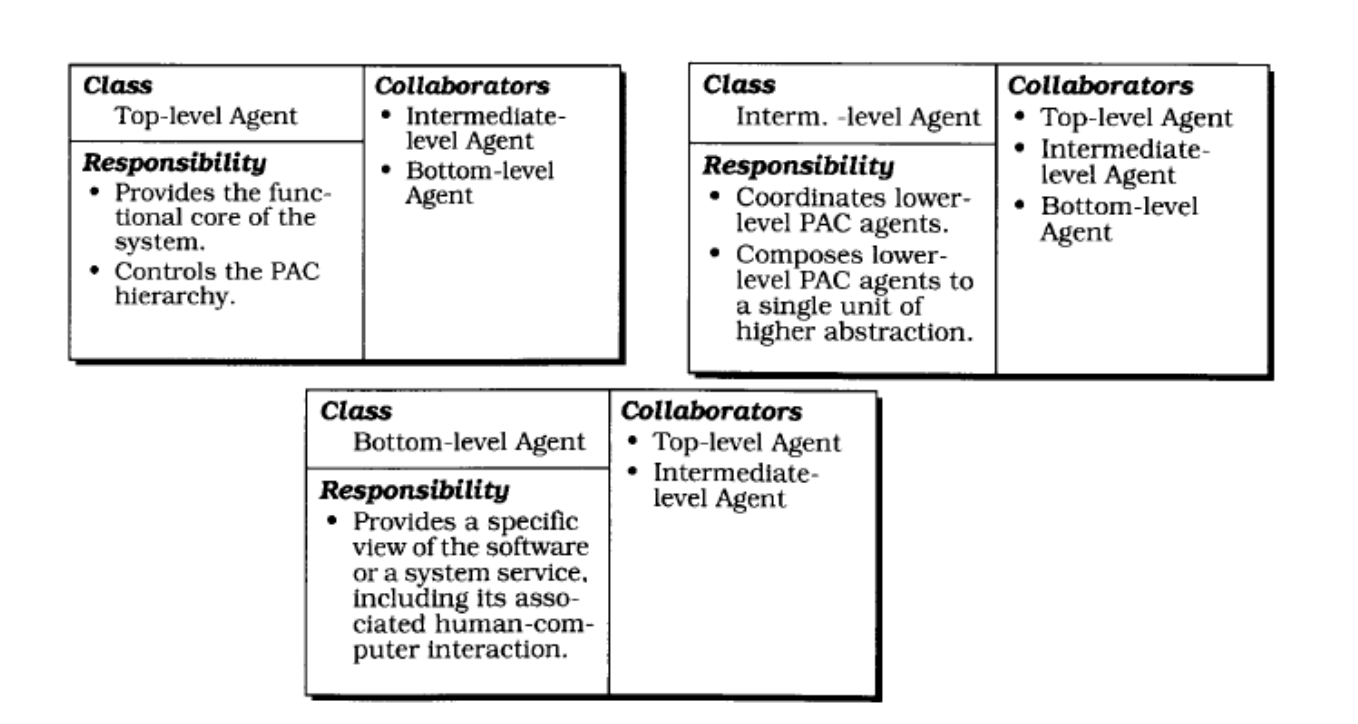
\includegraphics[width=.5\linewidth]{pac-struktura.png}
\end{figure}

    Zastosowania: Network Trafic Management (gathering traffic datha, displaying various user-configurable
    views of the whole network)

\subsubsection{Architektura filtry i potoki}

Każdy z podsystemów realizuje przetwarzanie danych
otrzymanych od innych podsystemów. Filtry i potoki
pozwalają na uporządkowanie systemu, który przetwarza strumienie danych.
Każdy krok przetwarzania jest zamknięty w filtrze. Dane są przesyłane za pomocą potoków.


\begin{figure}[h]
    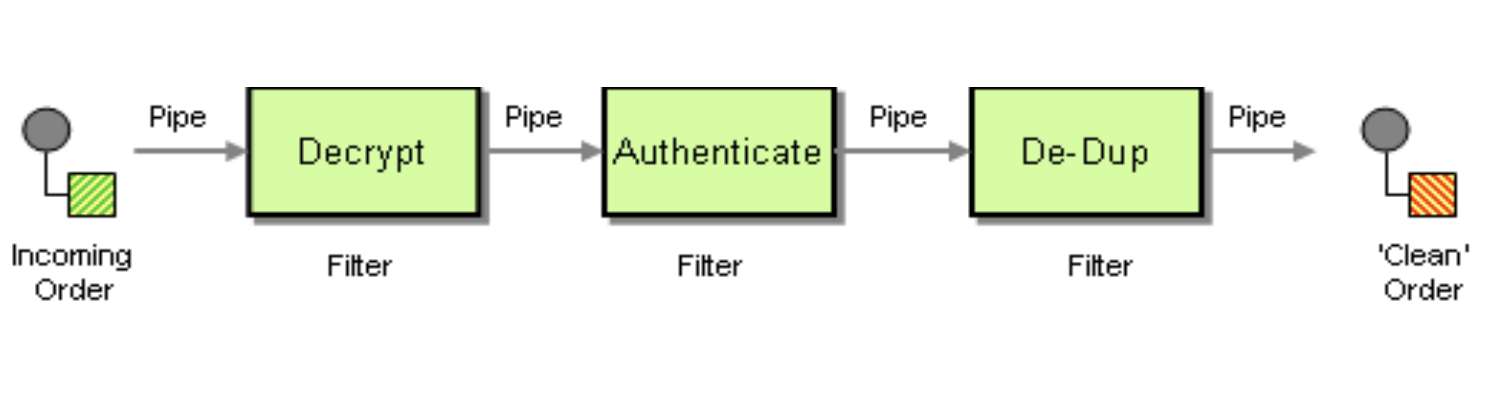
\includegraphics[width=.5\linewidth]{fip.png}
    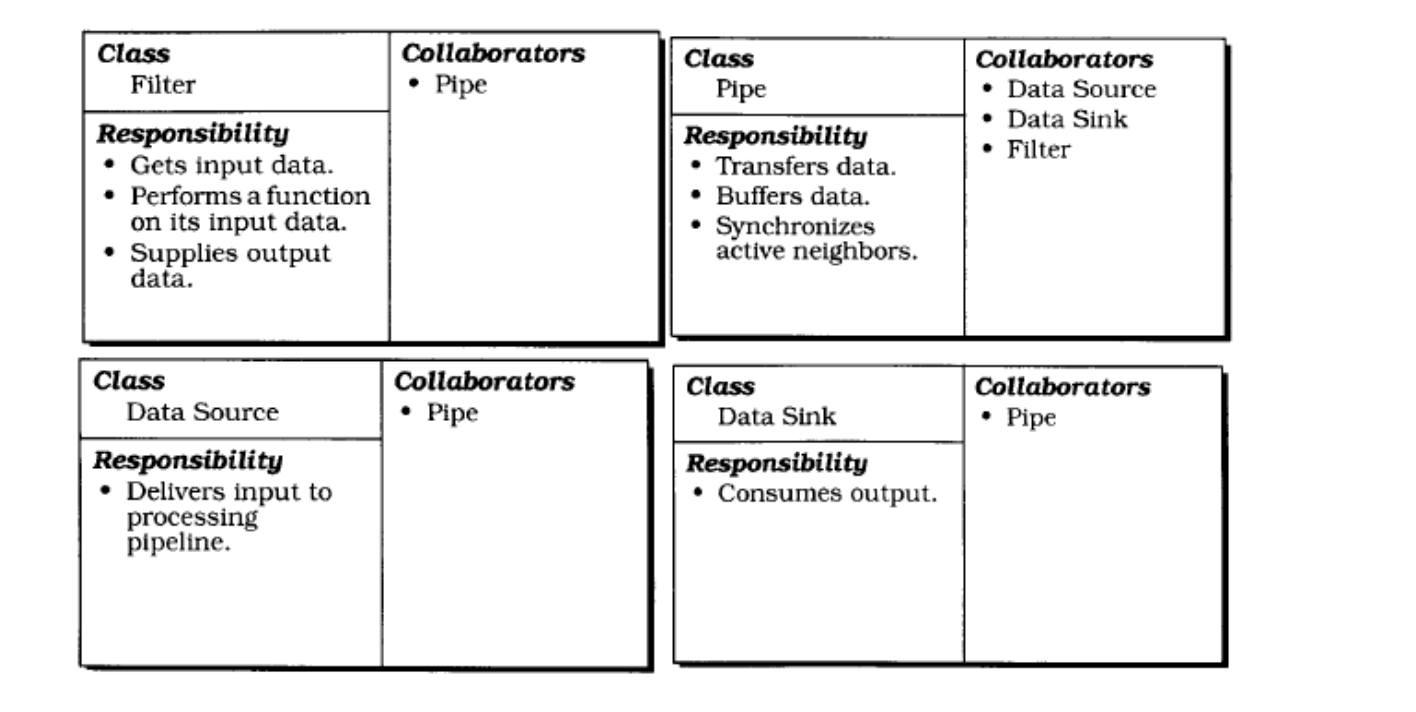
\includegraphics[width=.5\linewidth]{fip_struktura.png}
\end{figure}


Zastosowania: Unix, WEB, Servlet, Numerical Analysis (filters and data extractions)

\subsubsection{Tablica(blackboard)}
Jest użyteczna w systemach, gdzie nie są znane deterministyczne
rozwiązania danego problemu. W przypadku tablicy kilka wyspecjalizowanych
systemów łączy swoja wiedze w taki sposób, żeby stworzyć częściowe lub
przybliżone rozwiązanie problemu.


\begin{figure}[h]
    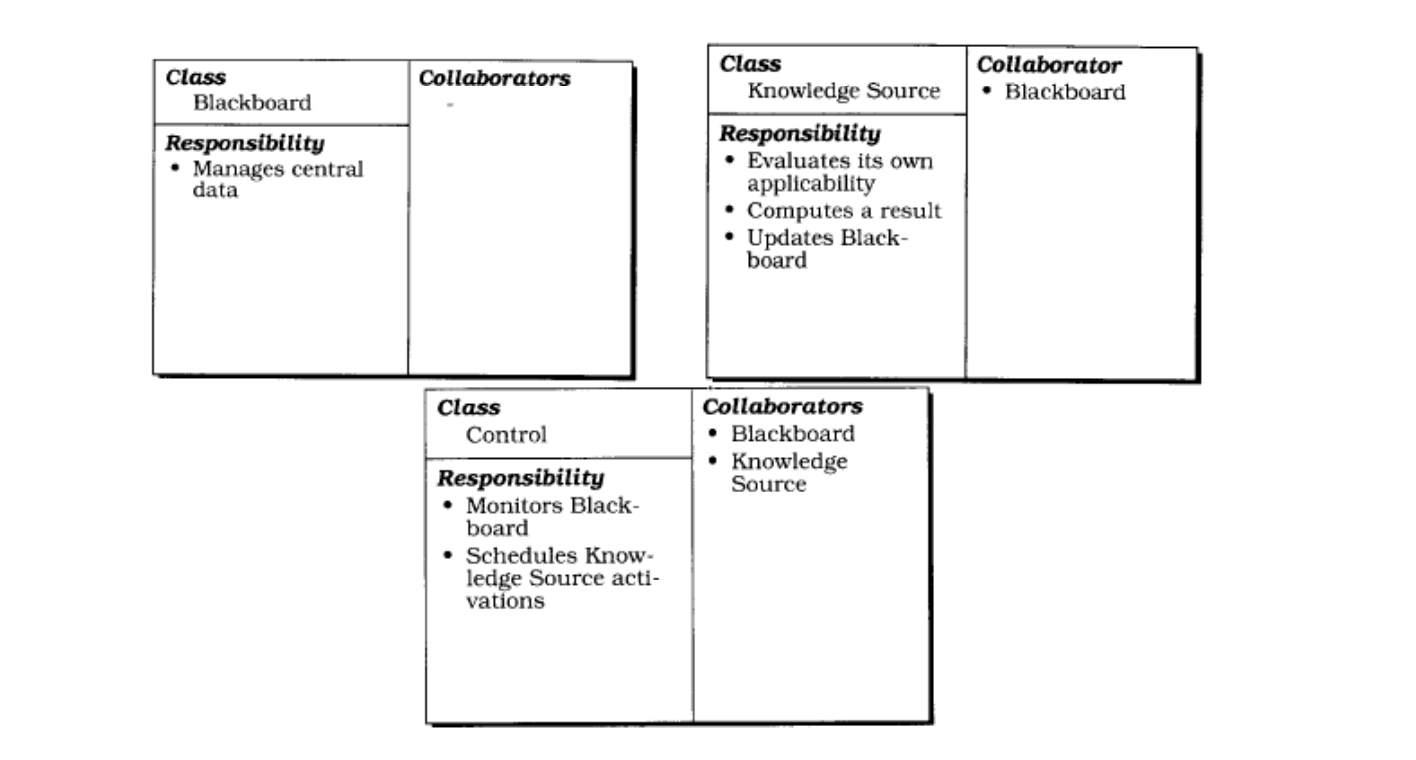
\includegraphics[width=.5\linewidth]{tablica.png}
\end{figure}

Zastosowania: working memory, repository data

\subsubsection{Broker}
Pozwala na uporządkowanie rozproszonych systemów podzielonych na
komponenty współpracujące ze sobą za pomocą zdalnego wywoływania
serwisu. Komponent brokera odpowiedzialny jest za koordynacje komunikacji.

\begin{figure}[h]
    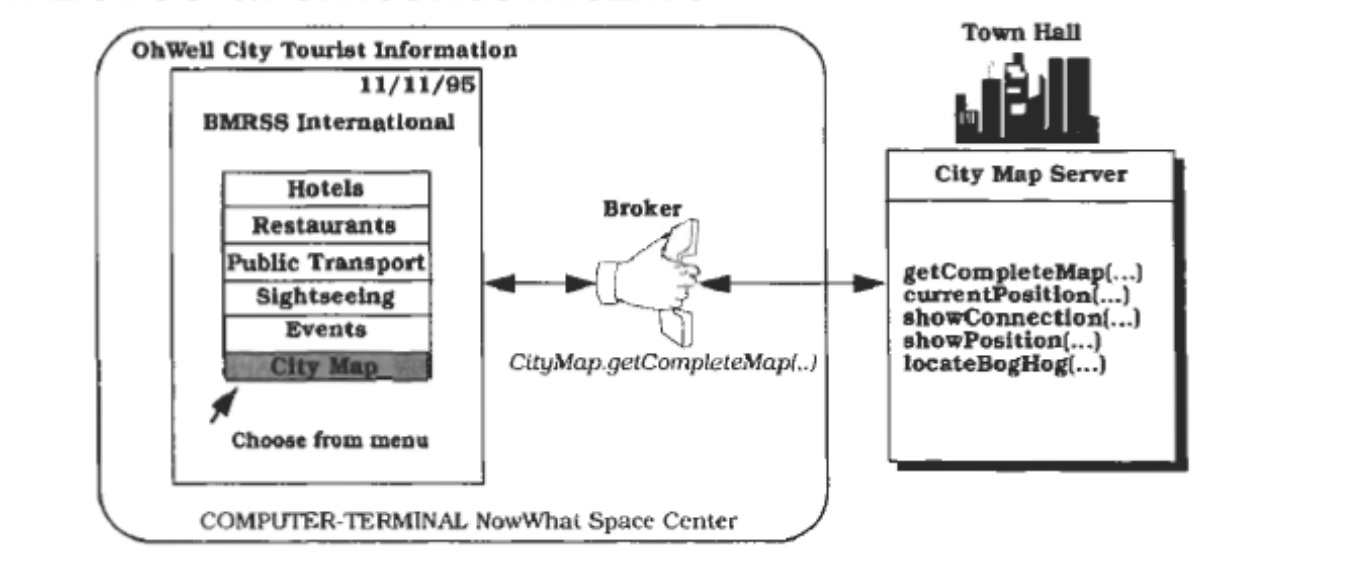
\includegraphics[width=.5\linewidth]{broker.png}
    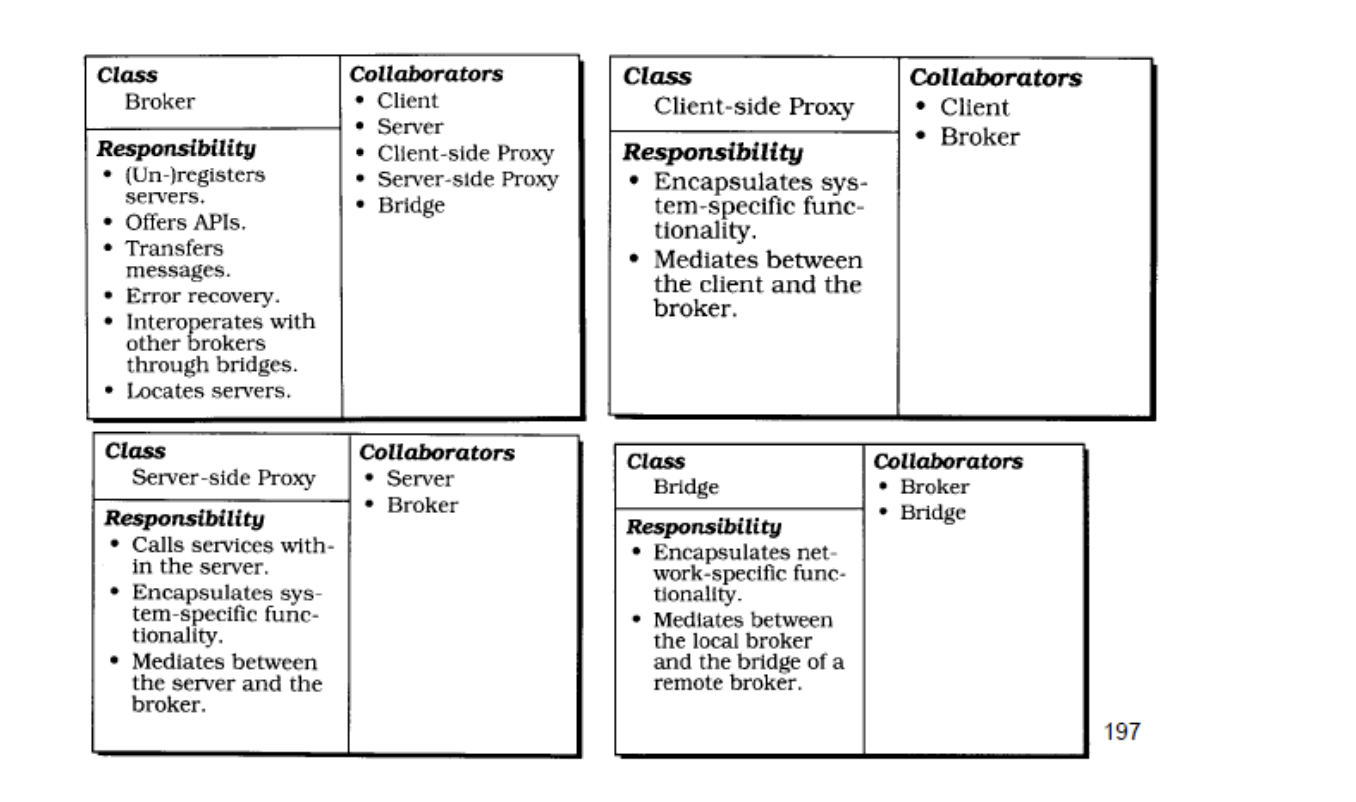
\includegraphics[width=.5\linewidth]{broker_struktura.png}
\end{figure}

\subsubsection{Reflection}
Dostarcza mechanizm pozwalający na dynamiczną zmianę zachowania
i struktury systemu informatycznego.
\begin{figure}[h]
    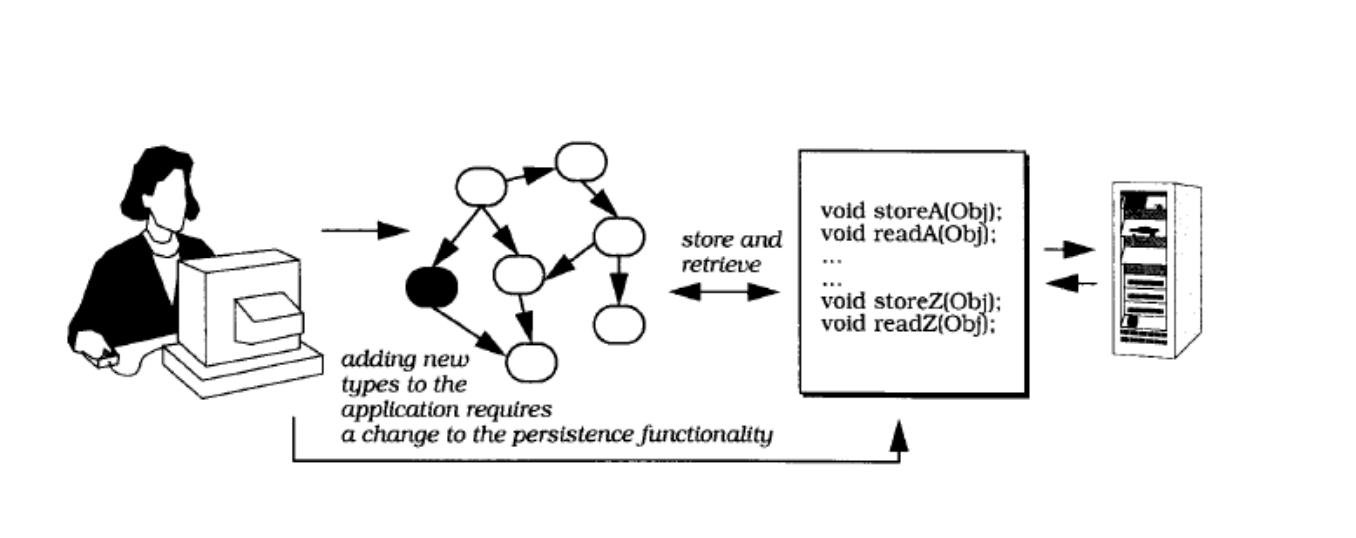
\includegraphics[width=.5\linewidth]{ref.png}
    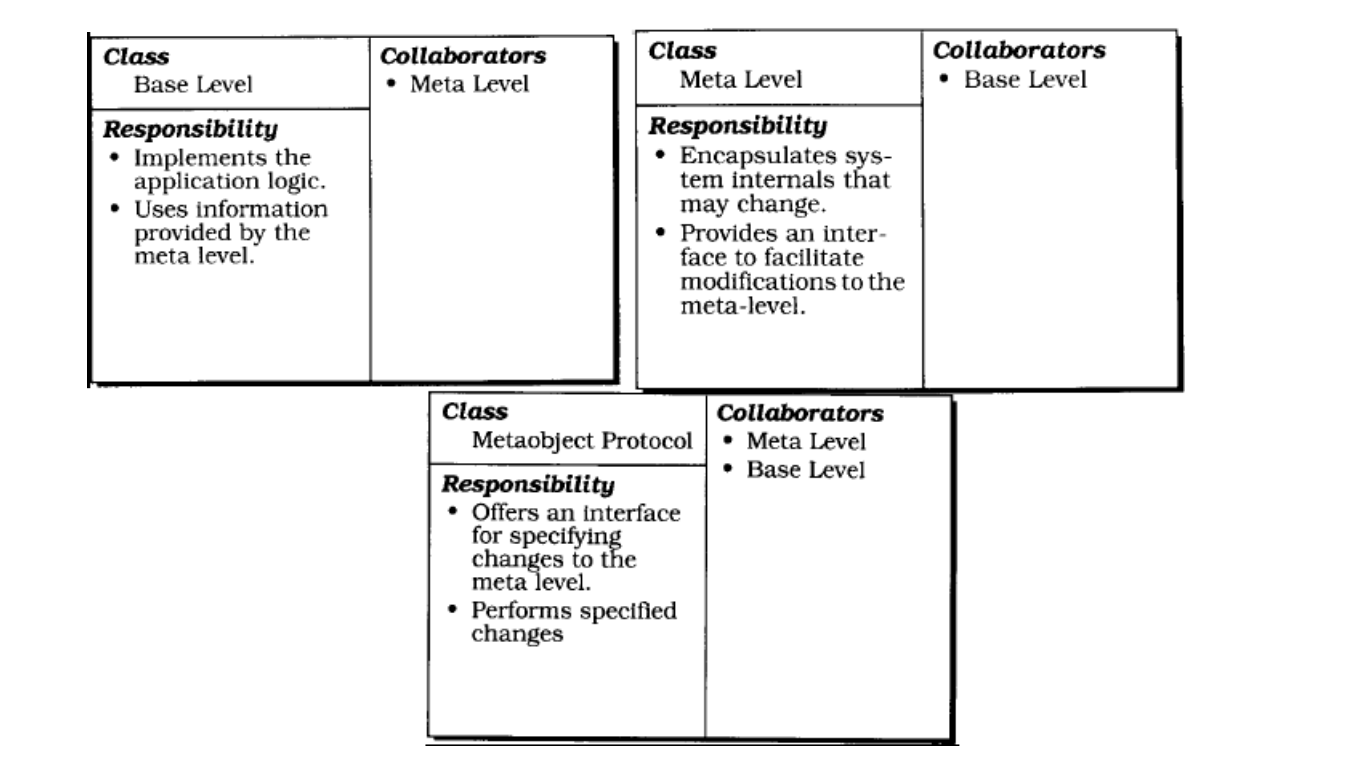
\includegraphics[width=.5\linewidth]{ref_struktura.png}
\end{figure}

Zastosowania: WWW.

\subsubsection{Sieciowe}
\begin{itemize}
    \item Architektura klient-serwer - podział systemu na dostawce usług (serwer) oraz ich odbiorców (klientów).
    \item Architektura peer-to-peer - każdy z podsystemów może spełniać obie funkcje (klient/serwer).

\end{itemize}

\subsubsection{Wzorce architektoniczne - wady}
    \begin{itemize}
        \item Patterns do not lead to direct code reuse.
        \item Individual Patterns are deceptively simple.
        \item Composition of different patterns can be very complex.
        \item Teams may suffer from pattern overload.
        \item Patterns are validated by experience and discussion
        rather than by automated testing.
        \item Integrating patterns into a software development
        process is a human-intensive activity.
    \end{itemize}


 \section{Projektowanie obiektów}
Projektowanie obiektów – ma na celu wypełnienie luki między obiektami
dziedziny aplikacyjnej a komponentami wybranymi na etapie projektowania systemu.


\begin{figure}[h]
    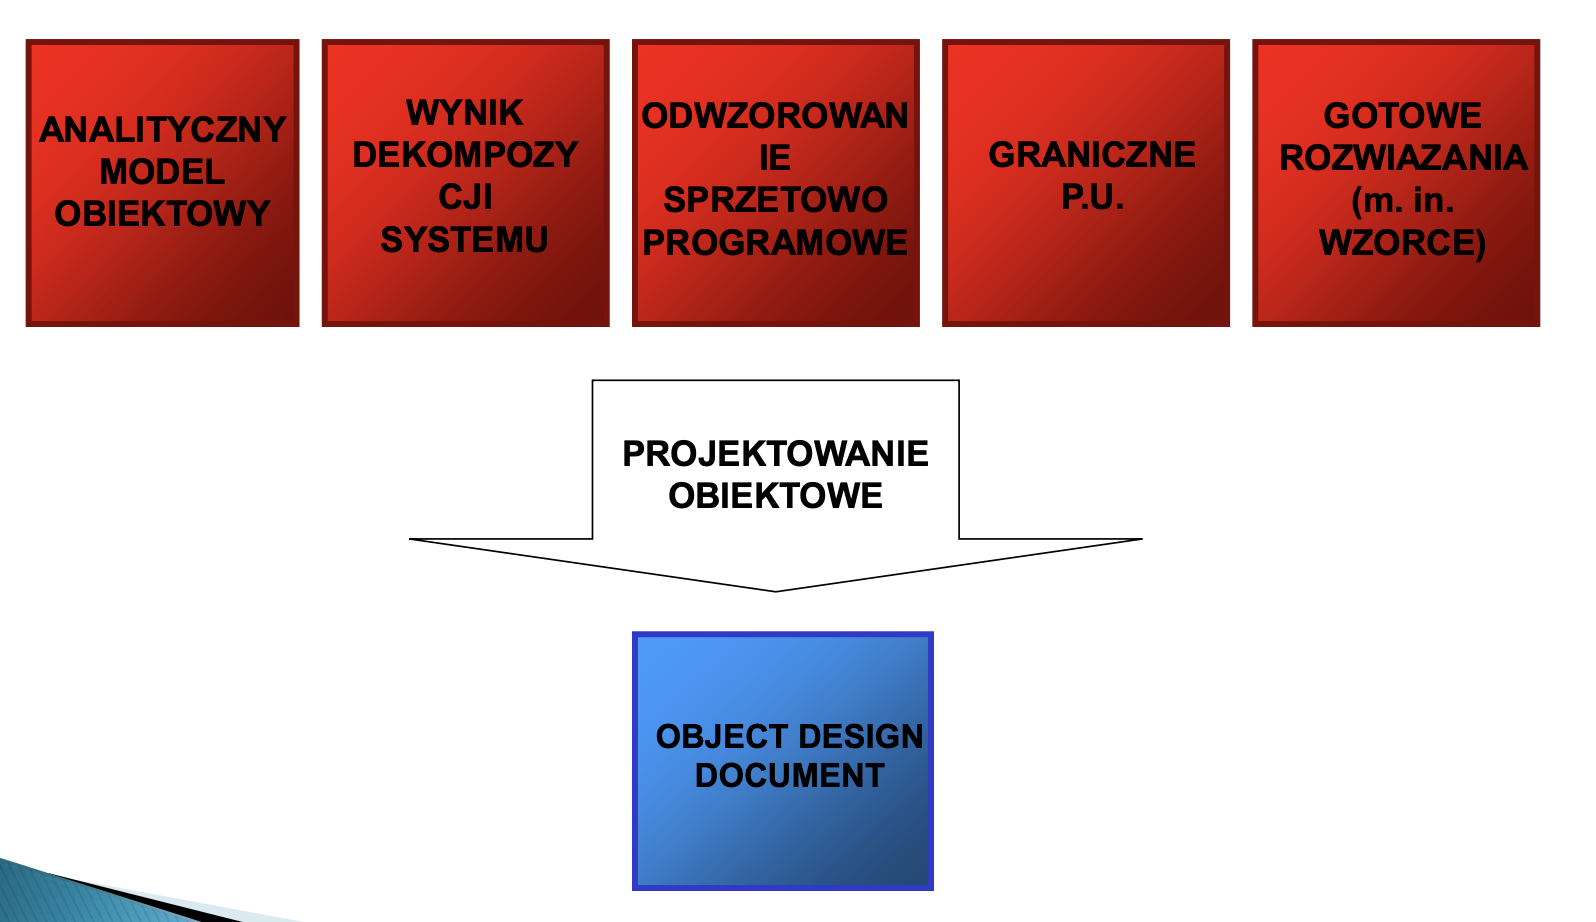
\includegraphics[width=\linewidth]{projektowanie_obiektow.png}
\end{figure}

Projektowanie obiektów można przedstawić w
postaci dekompozycji na następujące etapy:
\begin{itemize}
    \item wykorzystanie gotowych rozwiązań, którymi są zarówno
gotowe produkty (komponenty) jak i wzorce projektowe;
\item specyfikowanie usług;
\item restrukturyzacja modelu obiektowego;
\item optymalizacja modelu obiektowego;
\end{itemize}

\begin{figure}[h]
    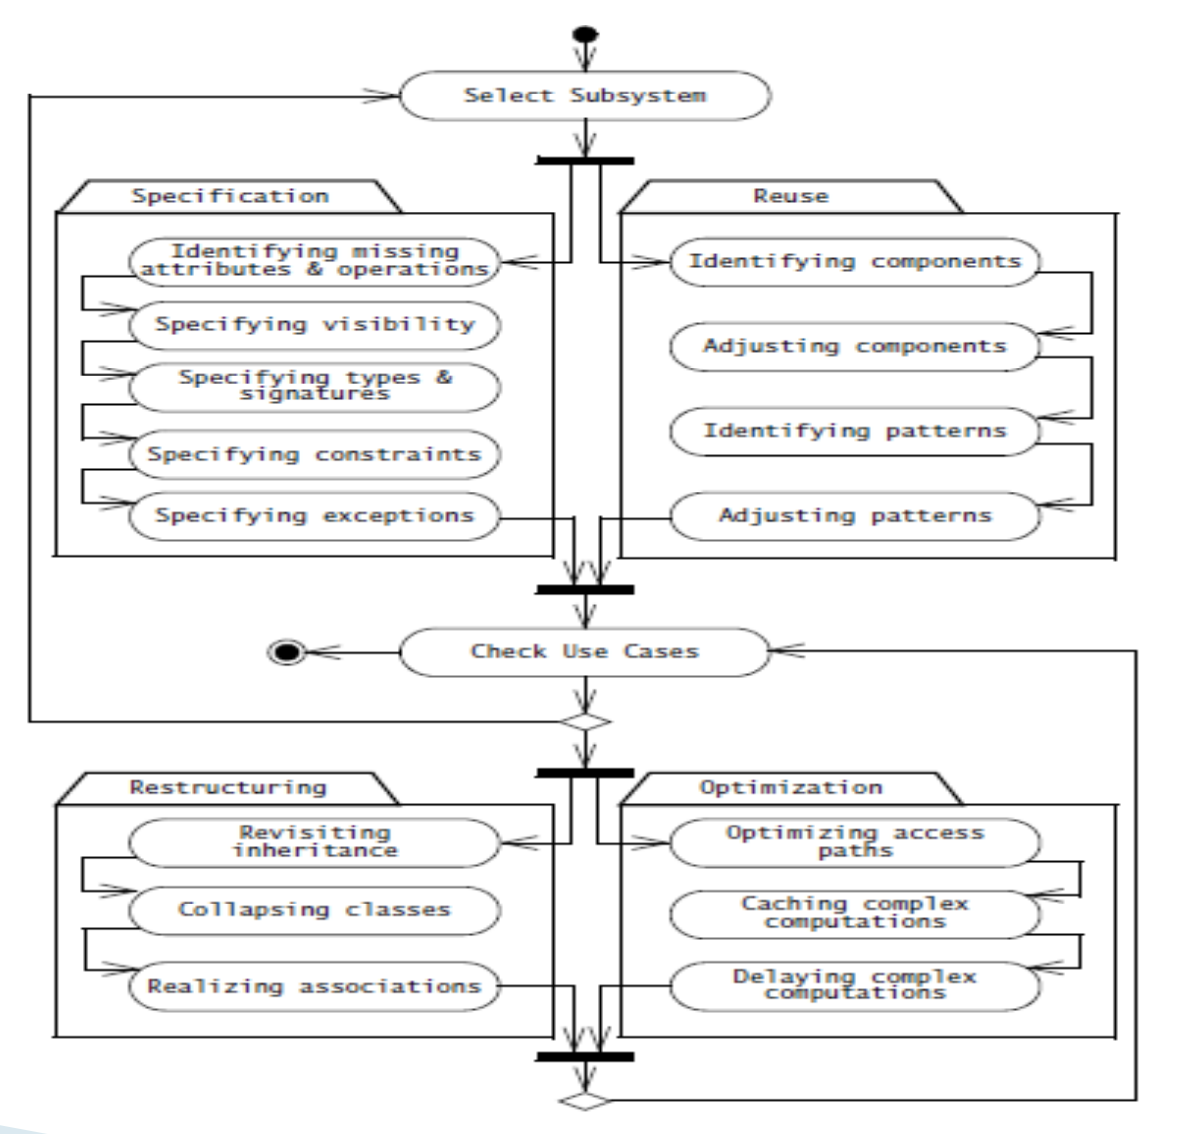
\includegraphics[width=\linewidth]{subsystem.png}
\end{figure}

Koncepcje wielokrotnego wykorzystywania
gotowych rozwiązań:
\begin{itemize}
    \item obiekty aplikacyjne i obiekty realizacyjne;
    \item dziedziczenie implementacyjne i dziedziczenie
specyfikacyjne;
    \item delegowanie;
    \item zasada zastępowania Liskov;
    \item wzorce projektowe (obiektowe);
\end{itemize}

Obiekty dziedziny aplikacyjnej reprezentują
koncepcje problemowe związane z tworzonym
systemem.

Obiekty realizacyjne reprezentują natomiast
komponenty nie mające odpowiedników w
dziedzinie aplikacyjnej, na przykład bazy danych
czy obiekty interfejsu użytkownika.

Dziedziczenie implementacyjne ma miejsce jeśli
sięgamy po dziedziczenie z zamiarem wykorzystania
gotowego kodu, mimo różnic koncepcyjnych
pomiędzy powiązanymi klasami.

Dziedziczenie specyfikacyjne ma odzwierciedlenie w
taksonomii klas (reprezentuje podtypowanie) - np. manager, pracownik etatowy, stażysta jako podtypy pracownika.

Alternatywą dla dziedziczenia implementacyjnego jest
delegowanie implementacji - zamiast implementować set jako nadpisywanie metod hashtable, implementujemy go jako set korzystajacy z instancji hashtable z własnymi metodami.
Delegowanie implementacji rozwiązuje
następujące problemy dziedziczenia
implementacyjnego:
\begin{itemize}
    \item rozszerzalność;
    \item podtypowanie;
\end{itemize}

\subsection{Zasada zastępowania Liskov}
    Jeśli obiekt klasy S może stać się substytutem obiektu klasy T w
    dowolnym miejscu kodu, w którym oczekiwany jest obiekt klasy T, to klasa S jest
    podtypem klasy T.

\subsection{Wzorce projektowe - poziom interakcji między klasami}
MOTYWACJA
    Różne dziedziny inżynierii stawiają sobie podobne pytania:
    \begin{itemize}
        \item Czy typowe problemy możan rozwiązać w powtarzalny sposób?
        \item Czy te problemy można przedstawić w sposób abstrakcyjny, tak aby były pomocne
        w tworzeniu rozwiązań w róznych konkretnych kontekstach?
    \end{itemize}

Wzorzec opisuje problem, który powtarza się wielokrotnie w danym środowisku, oraz podaje istotę
jego rozwiązania w taki sposób, aby możan było je zastosować milion razy bez potrzeby powtarzania
tej samej pracy.


\begin{itemize}
    \item Wzorce kreacyjne
    \begin{itemize}
        \item abstrakcyjne metody tworzenia obiektów
        \item uniezależnienie systemu od sposobu tworzenia obiektów
    \end{itemize}
    \item Wzorce strukturalne
    \begin{itemize}
        \item sposób wiązania obiektów w struktury
        \item właściwe wykorzystanie dziedziczenia i kompozycji
    \end{itemize}
    \item Wzorce behawioralne
    \begin{itemize}
        \item algorytmy i przydział odpowiedzialności
        \item opis przepływu kontroli i interakcji
    \end{itemize}
\end{itemize}

\subsection{Koncepcje specyfikowania interfejsów}
\begin{itemize}
    \item implementator (realize class), ekstender (refine class) i użytkownik (use class) klasy;
    \item typy, sygnatury (wektory/krotki typów parametrów i typu wyniku) i widzialność (public, private, protected, packet);
    \item kontrakty: niezmienniki, warunki wstępne i warunki końcowe;
    \item język OCL (Object Constraint Language) – ograniczenia
    \item OCL – zbiory, wielozbiory i ciągi;
    \item kwantyfikatory OCL;
\end{itemize}

\subsection{Aktywności specyfikowania interfejsów}
\begin{itemize}
    \item identyfikowanie brakujących atrybutów i operacji;
    \item definiowanie widzialności i sygnatur;
    \item specyfikowanie kontraktów;
    \item dziedziczenie kontraktów;
\end{itemize}



\subsection{SOLID}


\begin{tabular}{|c|c|}
    \hline
S & Single responsibility principle\\
& Klasa powinna mieć pojedyńczą
odpowiedzialność.\\
\hline
O & Open/closed principle\\
& Software powinien być otwarty na
rozszerzenia a zamknięty na modyfikacje.\\
    \hline
L & Liskov substitution principle\\
    \hline
I & Interface segregation principle\\
& Kilka konkretnych interfejsów jest lepszych
niż jeden ogólny\\
    \hline
D & Dependency inversion principle\\
& Software powinien zależeć od abstrakcji a
nie od konkretyzacji.\\
    \hline
\end{tabular}

\subsubsection{Single Resposibility Principle - SRP}
\begin{itemize}
    \item Nigdy nie powinien istnieć więcej niż jeden powód do modyfikacji klasy.
    \item Im mniejsza i bardziej wyspecyfikowana klasa tym łatwiej ją nazwać.
    \item Łatwiejsze wprowadzanie zmian.
    \item Łatwiejsze testowanie i naprawa
\end{itemize}

    Jak rozpoznać naruszenie SRP?
    \begin{itemize}
        \item Ilość linii kodu ( Class:LOC > 250)
        \item Za dużo
        zależności
        \item Słaba spojność
        \item Opis lub nazwa wymaga “i”
        \item Dużo zagnieżdżeń (ifów)
        \item Wymaga skomplikowanych testów
        \item Modyfikacja może zepsuć inne testy
    \end{itemize}



\subsubsection{Zasada otwarte-zamknięte}
    \begin{itemize}
        \item klasa powinna być otwarta na rozbudowę, ale zamknięta do jej własnej modyfikacji
        \item możemy dodawać nowe pola i metody, ale bez zmiany w wewnętrznej strukturze
        \item zmiana istniejącej struktury może mieć wpływ na inne elementy
        \item hermetyzacja, dziedziczenie, polimorfizm, delegaty
        \item unikamy instrukcji warunkowych
    \end{itemize}

\subsubsection{Zasada segregacji interfejsów}
\begin{itemize}
    \item Związki między klasami powinny być ograniczone do minimum
    \item Klient klasy powinien mieć dostep tylko do tyh składowych klasy,
    których rzeczywiście potrzebuje
    \item Moduły wysokiego poziomu nie powinny
    zależeć od modułów niskopoziomowych.
    \item Obie grupy modułów powinny zależeć od
    abstrakcji
\end{itemize}

\subsubsection{Zasada odwracania zależności}
'Hollywood Principle' - don't call us, we'll call you!

\subsection{Wybrane wzorce kreacyjne}

    \subsubsection{Singleton}
Cel:
    \begin{itemize}
        \item Zapewnienie, że klasa posiada jedną instancję wewnątrz całej aplikacji
        \item Stworzenie punktu dostępowego do tej instancji
    \end{itemize}

\begin{figure}[!h]
    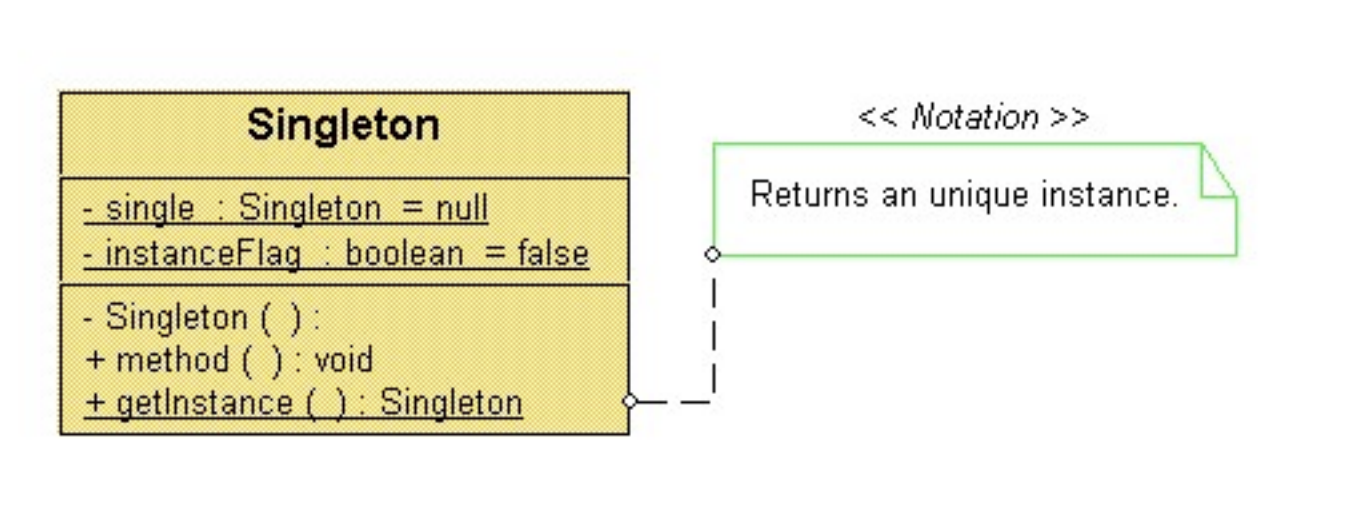
\includegraphics[width=\linewidth]{singleton.png}
\end{figure}

    \subsubsection{Factory method}
    Cel:
    \begin{itemize}
        \item Zdefiniowanie interfejsu do tworzenia obiektów
        \item Umożliwienie przekazania odpowiedzialności za tworzenie obiektów
        do podklas
        \item Umożliwienie wyboru klasy i konstruktora użytego do utworzenia
        obiektu
\end{itemize}

\begin{figure}[!h]
    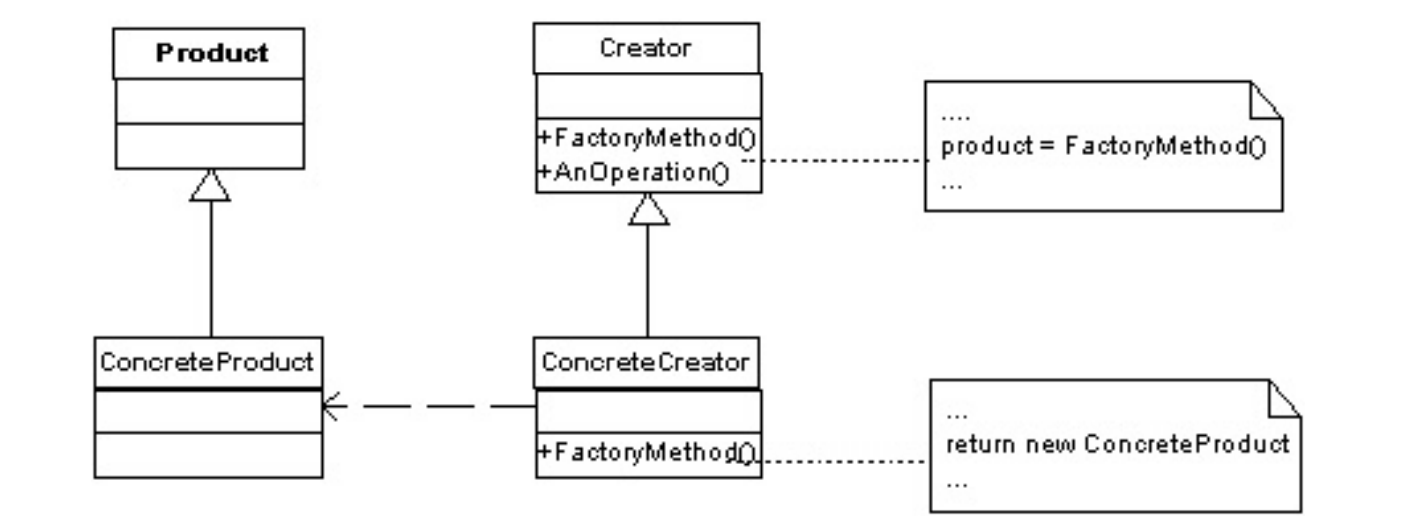
\includegraphics[width=\linewidth]{fac-met.png}
\end{figure}


    \subsubsection{Builder}
    Cel:
    \begin{itemize}
        \item Odseparowanie sposobu reprezentacji i metody konstrukcji
        złożonych struktur obiektowych
        \item Wykorzystanie jednego mechanizmu konstrukcyjnego do tworzenia
        struktur o różnej reprezentacji
\end{itemize}


\begin{figure}[!h]
    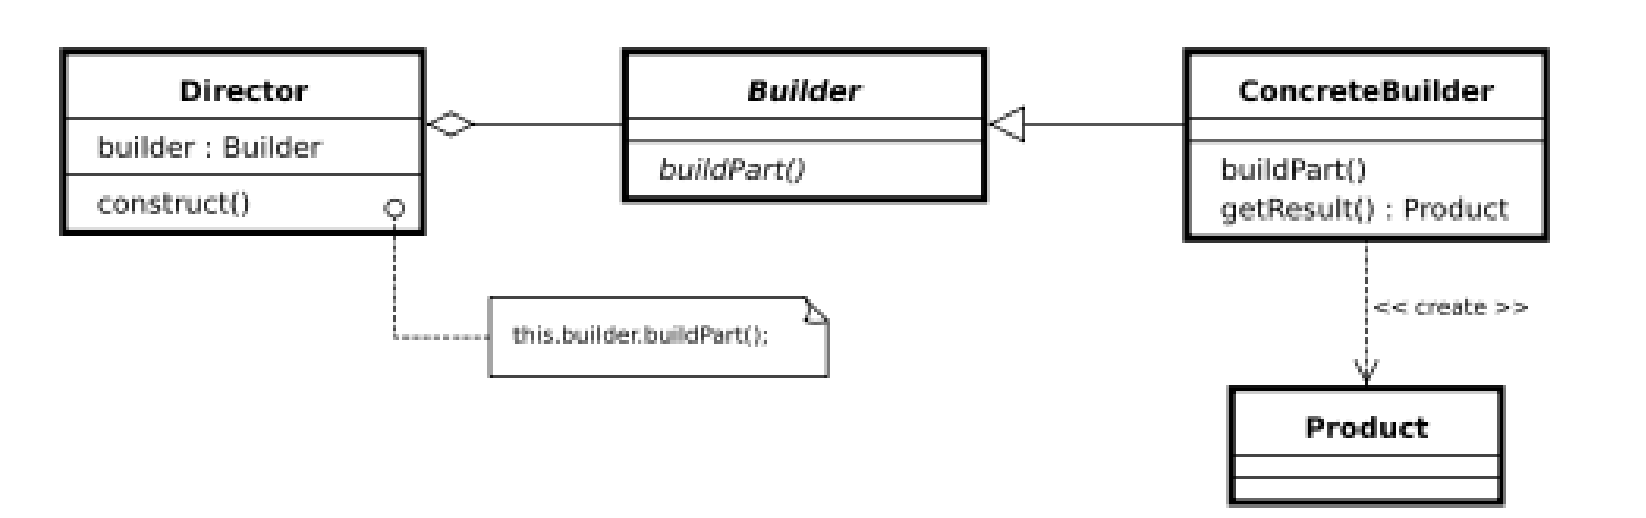
\includegraphics[width=\linewidth]{builder.png}
\end{figure}



\subsection{Wybrane wzorce strukturalne}

    \subsubsection{Adapter}
    Cel:
    \begin{itemize}
        \item Umożliwia współprace obiektów o niezgodnych typach
        \item Tłumaczy protokoły obiektowe
\end{itemize}

\begin{figure}[!h]
    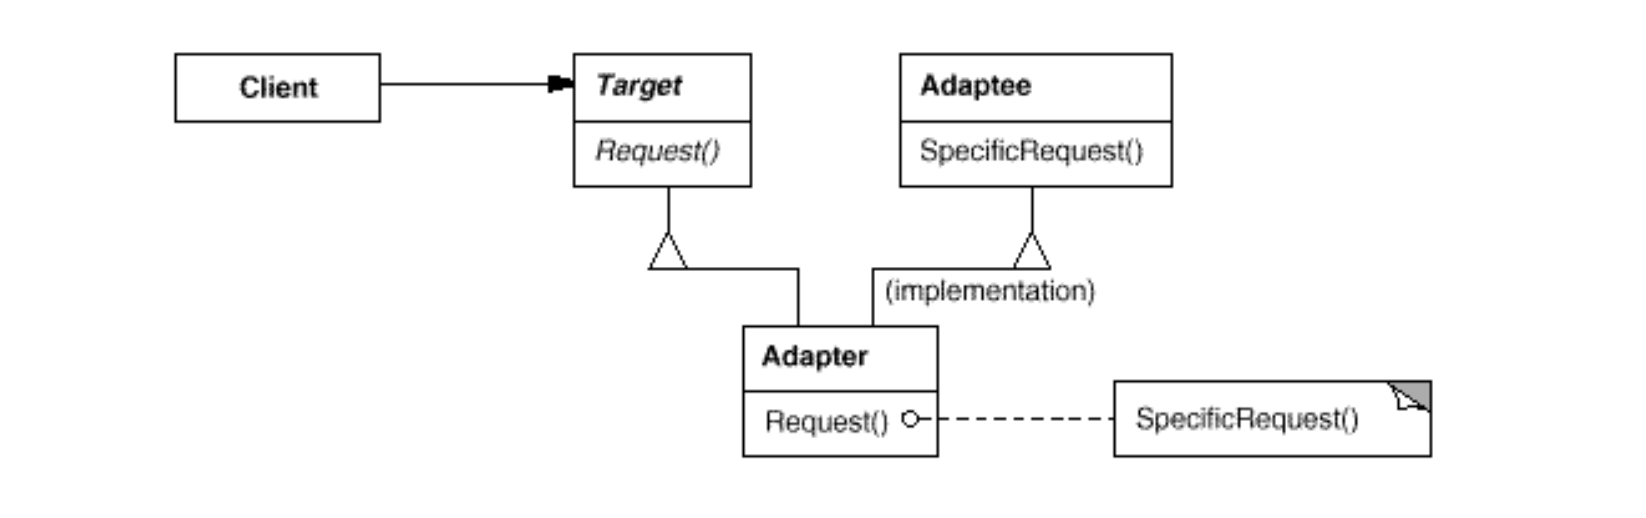
\includegraphics[width=\linewidth]{adapter.png}
\end{figure}

\subsubsection{Proxy}
    Cel:
    \begin{itemize}
        \item Dostarcza zamiennik obiektu w celu jego kontroli i ochrony
        \item Przezroczyste odsuniecie inicjalizacji obiektu w czasie
\end{itemize}

\begin{figure}[!h]
    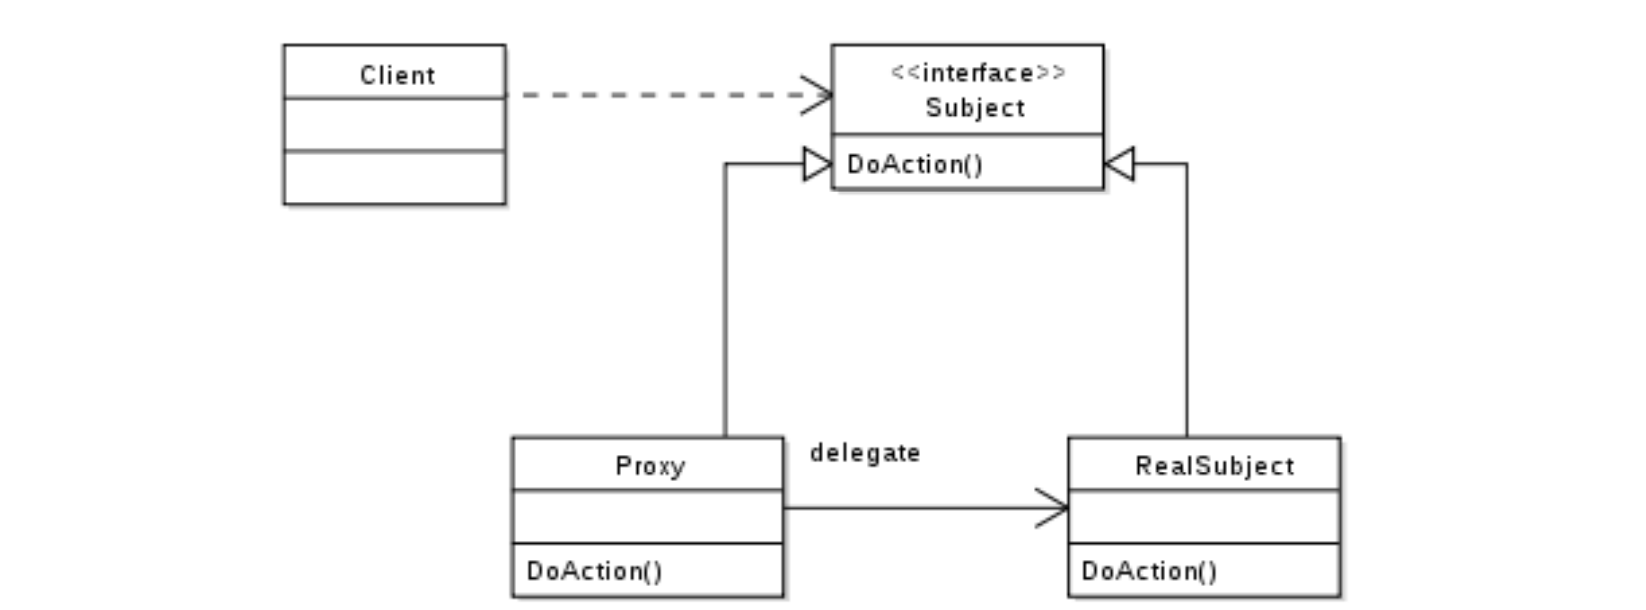
\includegraphics[width=\linewidth]{proxy.png}
\end{figure}



\subsubsection{Fasada}
    Cel:
    \begin{itemize}
        \item Dostarczenie jednorodnego interfejsu wyższego poziomu do zbioru
        rośnych interfejsów w systemie
        \item Ukrycie złożoności podsystemów przed klientem
\end{itemize}

\begin{figure}[!h]
    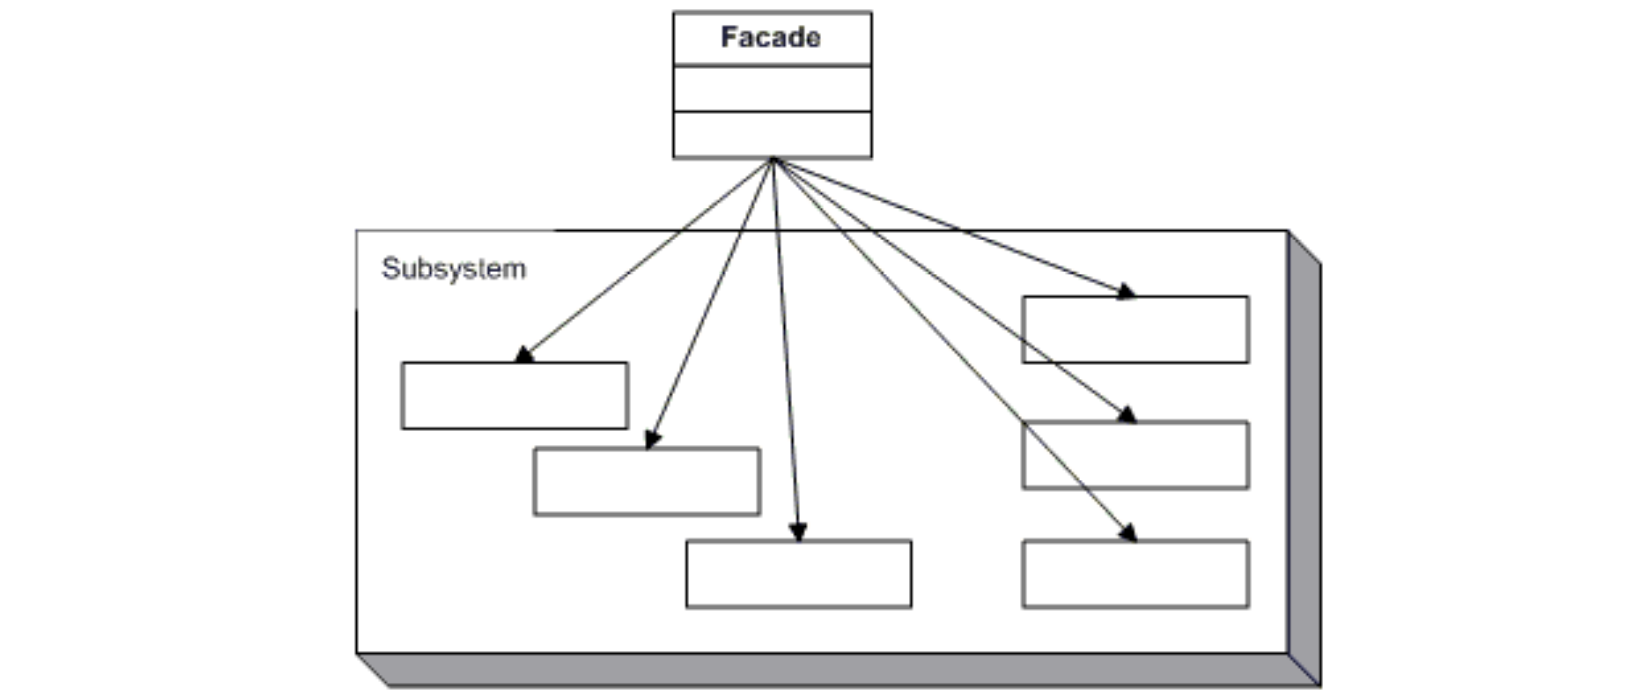
\includegraphics[width=\linewidth]{fasada.png}
\end{figure}




\subsection{Wybrane wzorce behawioralne}

    \subsubsection{Obserwator}
    \begin{itemize}
        \item Tworzy zależność typu jeden-wiele pomiędzy obiektami
        \item Informacja o zmianie stanu wyróżnionego obiektu jest przekazywana
        wszystkim pozostałym obiektom
    \end{itemize}

\begin{figure}[!h]
    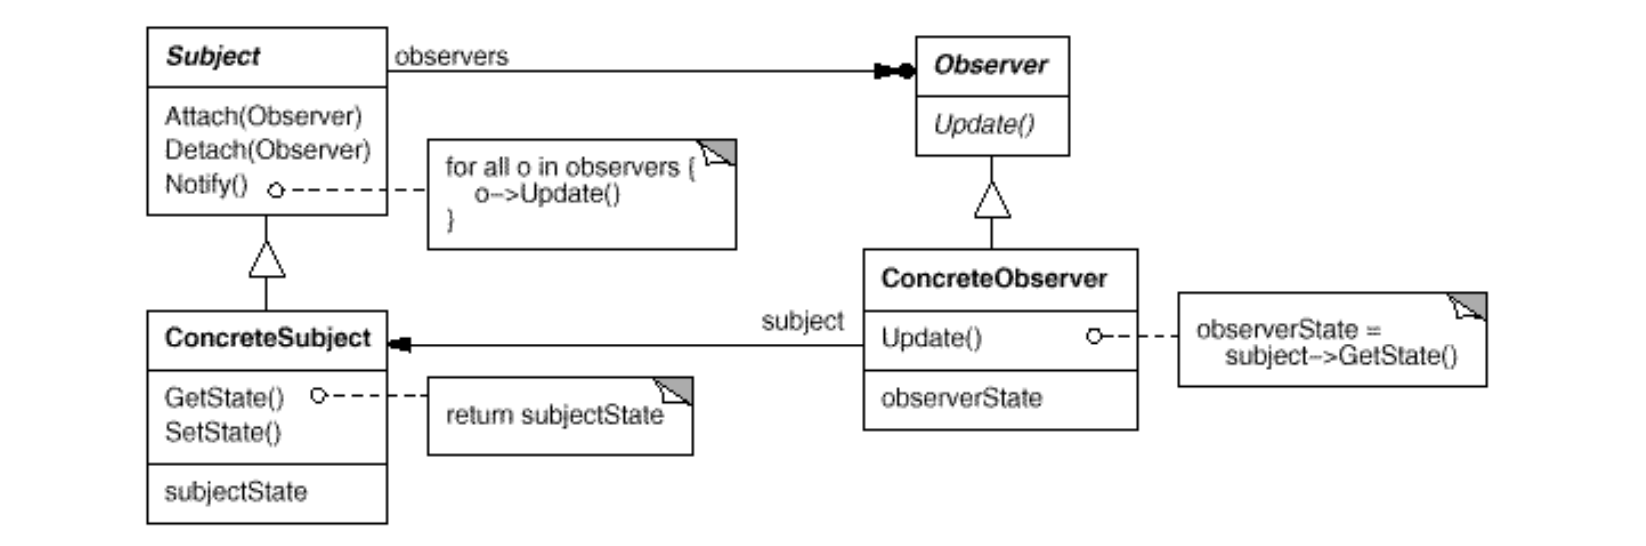
\includegraphics[width=\linewidth]{obserwator.png}
\end{figure}


\subsubsection{Command}
    \begin{itemize}
        \item Hermetyzacja poleceń do wykonania w postaci obiektów
        \item Umożliwienie parametryzacji klientów obiektami poleceń
        \item Wsparcie dla poleceń odwracalnych
    \end{itemize}

\begin{figure}[!h]
    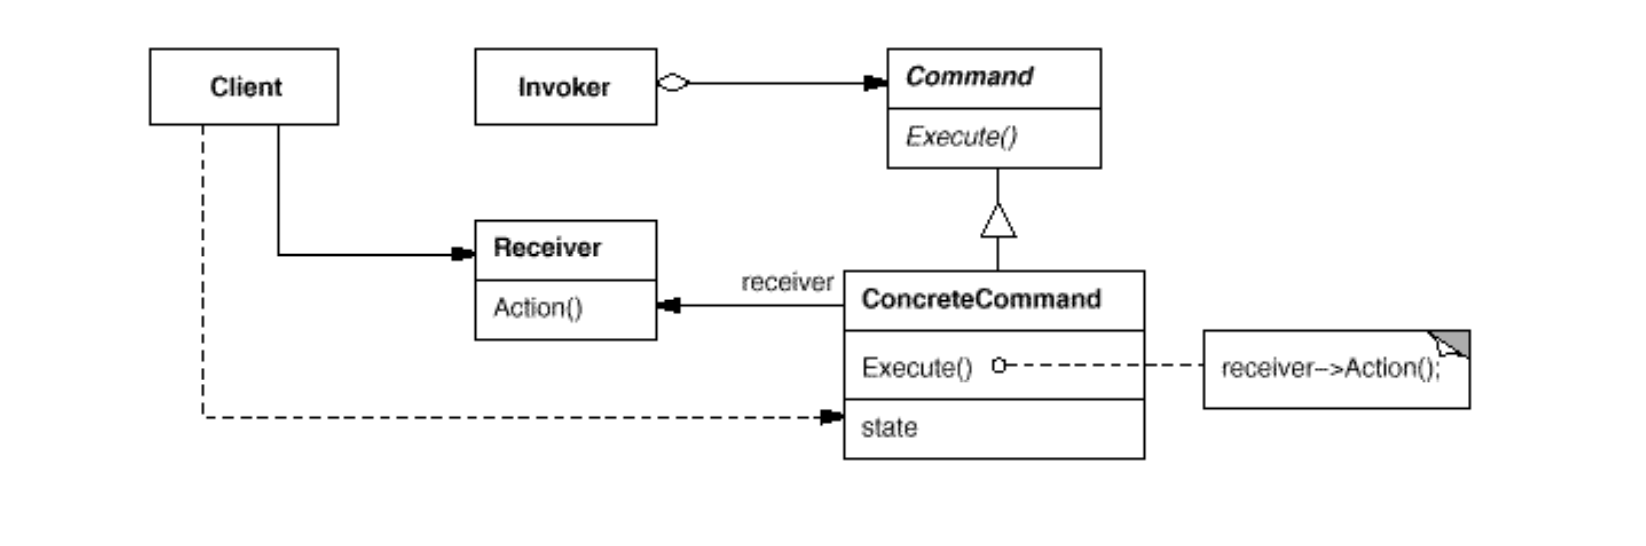
\includegraphics[width=\linewidth]{command.png}
\end{figure}


    \subsubsection{Chain of responsibility}
    Cel:
    \begin{itemize}
        \item  Usunięcie powiązania pomiędzy nadawcą i odbiorcą żądania
        \item Umożliwienie wielu obiektom obsługi żądania
    \end{itemize}


\begin{figure}[!h]
    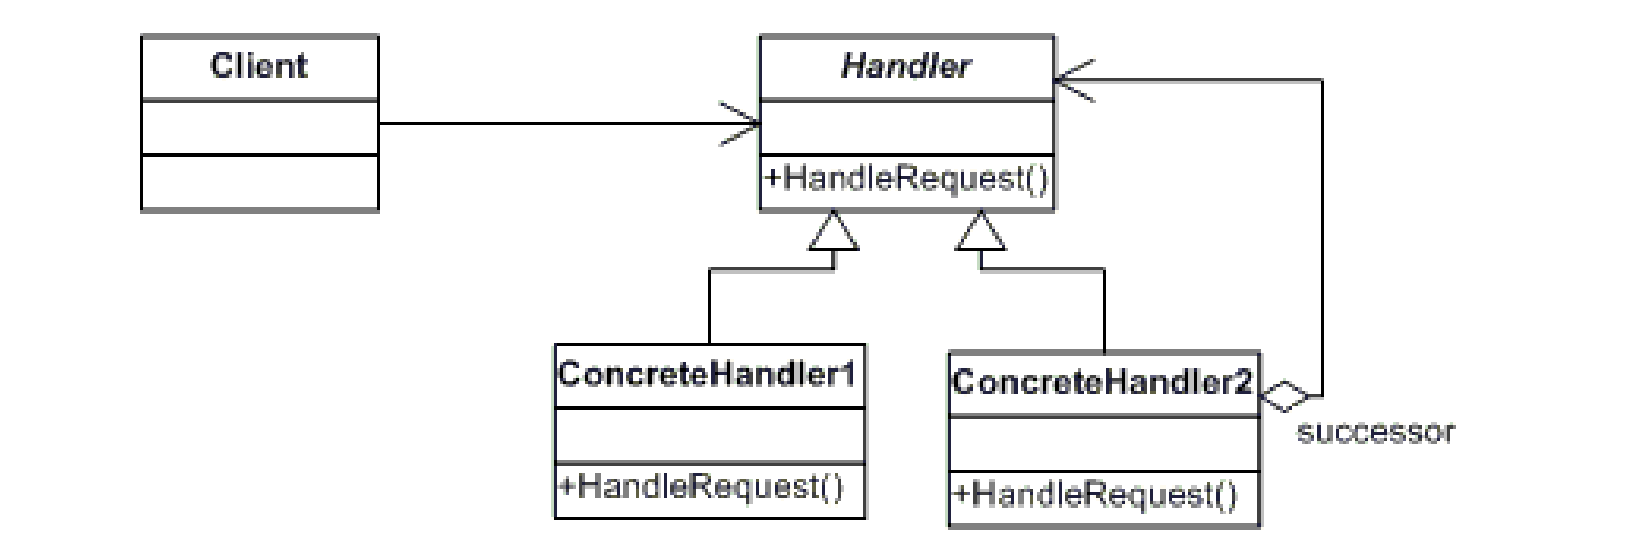
\includegraphics[width=\linewidth]{ch-o-r.png}
\end{figure}


    \subsubsection{Iterator}
    Cel:
    \begin{itemize}
        \item Umożliwienie sekwencyjnego dostępu do elementów kolekcji bez
        ujawniania jej wewnętrznej implementacji
    \end{itemize}





\begin{figure}[!h]
    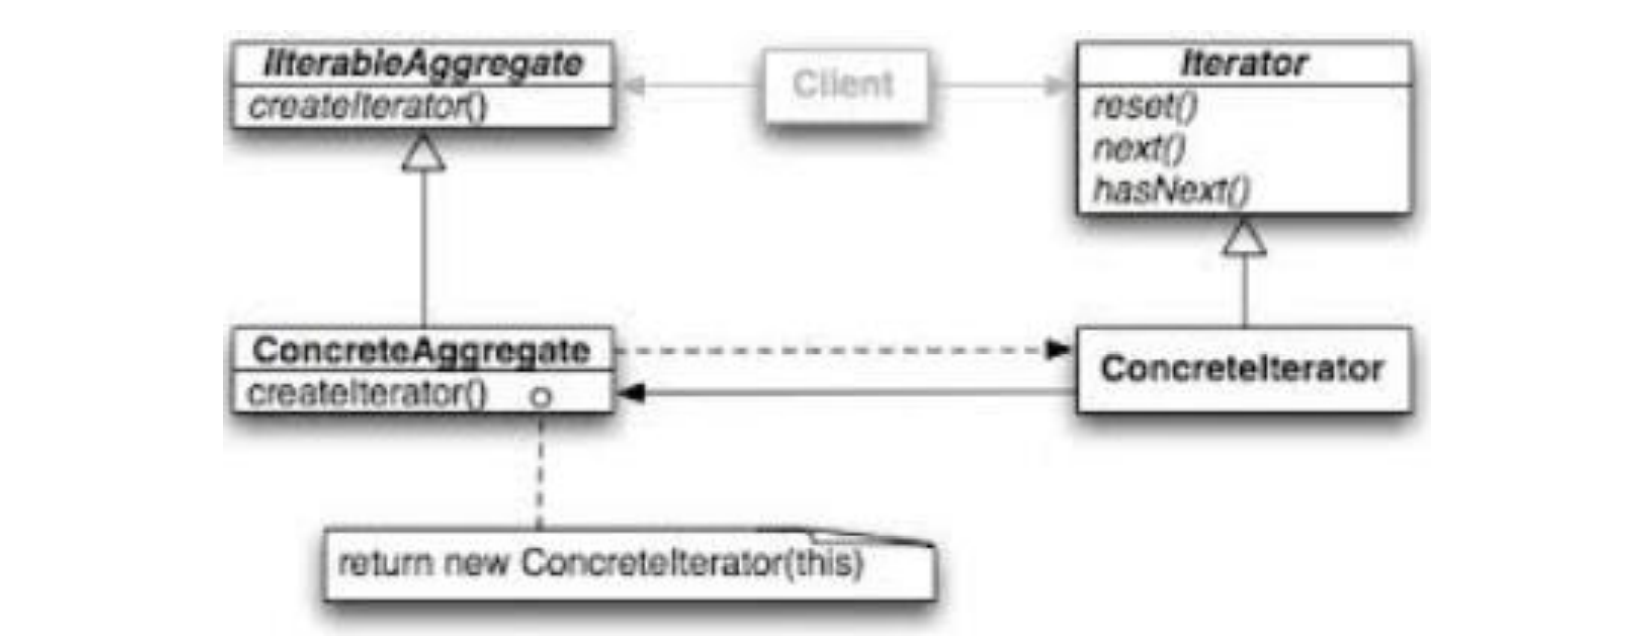
\includegraphics[width=\linewidth]{iterator.png}
\end{figure}



\subsection{Implementacja wzorców projektowych}
Implementacja to transformowanie modelu w kod źródłowy.



\begin{figure}[!h]
    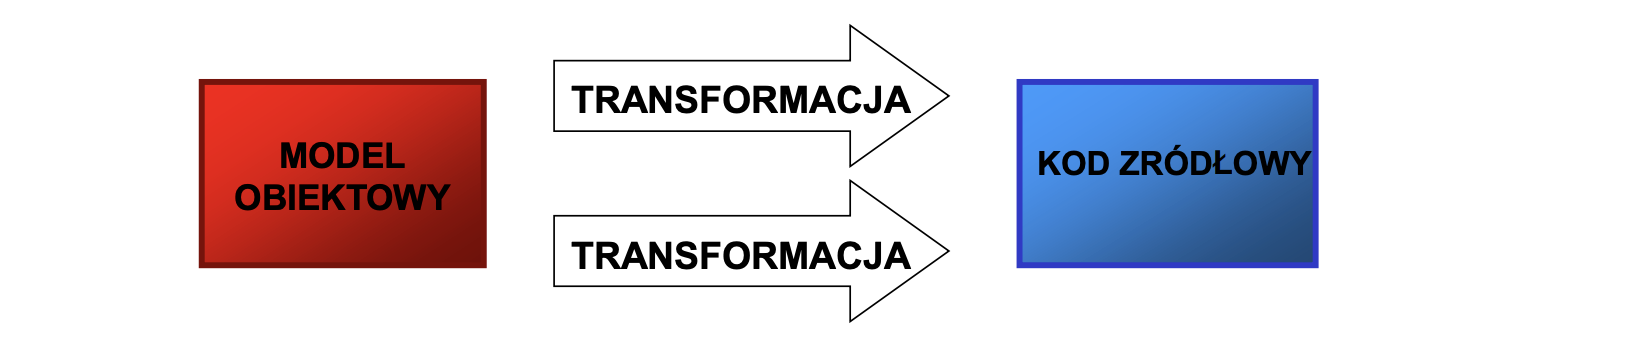
\includegraphics[width=\linewidth]{wzorce.png}
\end{figure}

Transformacje te wykonywane są w ramach następujących
aktywności:
\begin{itemize}
    \item optymalizowanie modelu
    \item realizowanie skojarzeń
    \item definiowanie wyjątków związanych z naruszeniem kontraktów
    \item odwzorowywane modeli klas w schematy przechowywania danych
\end{itemize}

Zasady transformacji:
\begin{itemize}
    \item każda transformacja powinna dotyczyć tylko jednego,
    ściśle określonego kryterium;
    \item każda transformacja musi mieć charakter lokalny;
    \item każda transformacja powinna być izolowana od
    innych zmian;
    \item każda transformacja musi być poddana weryfikacji;
\end{itemize}


Najczęściej wykonywane aktywności (transformacje):
\begin{itemize}
    \item optymalizowanie modelu obiektowego;
    \item odwzorowywanie skojarzeń w kolekcje;
    \item odwzorowywanie kontraktów w wyjątki;
    \item odwzorowywanie modelu obiektowego w schematy
    bazy danych;
\end{itemize}

Typy transformacji
    \begin{itemize}
        \item Transformacja modelu
        \begin{itemize}
            \item ograniczona jest do samego modelu
            \item celem jest uproszczenie lub zoptymalizowanie istniejącego modelu
        \end{itemize}
        \item Inżynieria postępująca
        \begin{itemize}
            \item tworzenie szablonów kodu źródłowego odpowiadającego modelowi obiektowemu
        \end{itemize}
    \end{itemize}

\subsubsection{Paradygmaty programowania}

Paradygmat:
\begin{itemize}
    \item wzorzec lub najogólniejszy
model lub jako wzorcowy przykład.
    \item zbiór pojęć i teorii tworzących podstawy danej nauki.
\end{itemize}


Podstawowe założenia paradygmatu:
    \begin{itemize}
        \item Abstrakcja\\
        System rozumiany jest jako układ obiektów . Każdy
        obiekt w systemie można rozpatrywać jako model
        abstrakcyjnego elementu, który może:
        \begin{itemize}
            \item opisywać i zmieniać swój stan,
            \item komunikować się z innymi obiektami w systemie,
            \item wykonywać pewne czynności na rzecz innych obiektów,
            \item bez ujawniania, w jaki sposób zaimplementowano
        dane cechy.
        \end{itemize}
        \item Enkapsulacja\\
        \begin{itemize}
            \item Polega na ukrywaniu szczegółów implementacji.
            \item Ma to spowodować, że obiekt nie może zmieniać
            stanu wewnętrznego innych obiektów w
            nieoczekiwany sposób.
            \item Tylko wewnętrzne metody obiektu są uprawnione
            do zmiany jego stanu.
            \item Każdy typ obiektu dostarcza innym obiektom swój
            "interfejs", który określa dopuszczalne metody współpracy.
        \end{itemize}
        \item Polimorfizm\\
        \begin{itemize}
            \item Polimorfizm w programowaniu obiektowym to
        wykazywanie różnych form działania podczas
        wywoływania metody w zależności od tego jakiego
        typu obiekt jest wskazywany przez wskaźnik lub
        referencję.
            \item Referencje i kolekcje obiektów mogą dotyczyć
        obiektów różnego typu, a wywołanie metody dla
        referencji spowoduje zachowanie odpowiednie dla
        pełnego typu obiektu wywoływanego.
        \end{itemize}
        \item Dziedziczenie\\
        \begin{itemize}
            \item Dziedziczenie porządkuje i wspomaga polimorfizm i
            enkapsulację.
            \item Osiąga to dzięki umożliwieniu definiowania i
            tworzenia specjalizowanych obiektów na podstawie
            bardziej ogólnych.
            \item Dla obiektów specjalizowanych nie trzeba
            redefiniować całej funkcjonalności, lecz tylko tę,
            której nie mają obiekty ogólniejsze.
        \end{itemize}
    \end{itemize}

GRASP - General Responsibility Assignment Software Patterns odpowiada na pytania w zakresie odpowiedzialności.
    \begin{itemize}
        \item Creator - określa kiedy podany obiekt powinien tworzyć inny obiekt, tzn. B powinien tworzyć A, jeśli:
        \begin{itemize}
            \item B agreguje A,
            \item B operuje na danych obiektu A,
            \item B używa bezpośrednio A,
            \item B dostarcza informacji niezbędnej do utworzenia A
        \end{itemize}
        \item Information Expert\\
        Programista powinien delegować nową
        odpowiedzialność (nowe funkcje) do obiektów, które
        zawierają najwięcej informacji/danych
        pozwalających zrealizować nową funkcjonalność.
        Istotne jest więc określenie, jakie dane są niezbędne
        do wypełnienia danej odpowiedzialności. Dopiero w
        tym momencie można powiedzieć, który obiekt
        powinien mieć przypisaną nową funkcjonalność
        \item Controller\\
        Programista powinien delegować zadania z interfejsu
        użytkownika do kontrolera.
        Zadaniem kontrolera jest: odbieranie informacji od UI,
        wykonywanie operacji oraz zwracanie ich wyników
        do UI. Kontroler powinien delegować zadania w głąb
        systemu
        \item Low Coupling\\
        Klasy powinny być od siebie jak najbardziej
        niezależne. Zmiana w jednej klasie powinna
        prowadzić do jak najmniejszej ilości zmian w innych
        klasach.
        \item High Cohesion\\
        Obiekt powinien skupiać się na jednej
        odpowiedzialności. Jego odpowiedzialność nie
        powinna być rozmyta, gdyż nie wiadomo
        wtedy dlaczego obiekt istnieje w systemie
        \item Polymorphism
        \item Pure Fabrication\\
        W systemie mogą istnieć operacje, których nie
        da się przypisać do żadnego obiektu
        dziedziny. Prowadzi to do powstawania w
        systemie obiektów, które nie reprezentują
        żadnego obiektu dziedziny, a kondensują
        funkcje udostępniane na rzecz innych
        obiektów.
        Zapewniają zbiór usług na rzecz innych
        obiektów, np.: dostęp do repozytorium.
        \item Indirection\\
        Aby zapewnić low coupling często zachodzi potrzeba
        dodania mediatora w komunikacji między biektami.
        Jego zadaniem jest jedynie wymiana informacji
        między obiektami. Taki obiekt deleguje zadania z
        jednego obiektu na rzecz drugiego. Projektowanie
        systemu z użyciem mediatora wpływa na poprawę
        hermetyzacji elementów systemu.
        Model MVC jest dobrym tego przykładem astosowania
        tej zasady. Kontroler jest mediatorem, co izoluje
        interfejs użytkownika od modelu.
        \item Protected variations\\
        Zasada mówiąca o zakresie modyfikacji w systemie
        wymaganym przez określoną zmianę. W systemie
        powinno się identyfikować punkty niestabilności i
        budować interfejsy wokół tych punktów.
        To ograniczy zakres zmian w przypadku, gdyby
        okazało się, że podany punkt niestabilności systemu
        wymaga zmian.
    \end{itemize}




\subsubsection{Metazasady}


\begin{itemize}
    \item Don't repeat yourself - DRY\\
    Jedno miejsce w systemie, na pojedynczą informację,
    co ułatwia późniejsze zmiany.
    Inna nazwa to Single Source Of Truth (SSOT), każda
    informacja w systemie powinna być przechowywana
    dokładnie raz, bo ułatwia to jej modyfikację.
    \item Keep it simple, stupid - KISS\\
    W projektowaniu interfejsów powyższą zasadę można
    nazwać zasadą najmniejszego zaskoczenia, czyli
    fragment kodu powinien robić dokładnie to co ma
    robić.
    Czasem trzeba wybrać, czy dany fragment kodu
    napisać z wykorzystaniem wzorca projektowego czy
    prostej konstrukcji.
\end{itemize}











\end{document}
